\section{Wstęp}
\suppressfloats[t]  %żeby obiekt ruchomy (rysunek, tablica, itp.) nie pojawił się u góry tej strony
\subsection{Cel i~zakres pracy}

Sprawdzenie możliwości wykorzystania internetu rzeczy, oraz bezzałogowych statków powietrznych, przy wspomaganiu prowadzenia akcji ratowniczej. Fizyczne zaprojektowanie i wykonanie kompletnego systemu, części działającej na pokładzie statku powietrznym, oraz części działającej na ziemi. Przetestowanie systemu w warunkach symulowanej akcji ratunkowej. Potwierdzenie lub zaprzeczenie użyteczności projektowanego systemu, wykazanie wad i zalet systemu.

\subsection{Tło projektu}

Pomysł projektu nasunęli organizatorzy konferencji "Parada Robotów 2017" i zarazem konkursu "Droniada" \cite{droniada}. Zadaniem uczestników konkursu było wspomaganie ewakuacji medycznej 10 osób po ataku huraganowego wiatru, przy użyciu bezzałogowców w locie autonomicznym, lub ewentualnie półautonomicznym, oraz tzw. beaconów \cite{beacon}. W tym dokumencie opiszę system lokalizowania poszkodowanych osób, który stworzyłem na potrzeby wspomnianego wyżej konkursu. Przejdę od projektu systemu, przez jego implementację, testy, oraz to jak sprawdził się w zadaniu konkursowym, na koniec przedstawię wnioski jakie wyciągnąłem z tego projektu i czy może on mieć jakąkolwiek przyszłość komercyjną. Poniżej na zdjęciu znajduje się część naszego zespołu która brała udział w konkursie "Droniada", wraz z płatowcem użytym w misji konkursowej \ref{fig:zespoldroniada}.

\begin{figure}[!th]
    \centering
    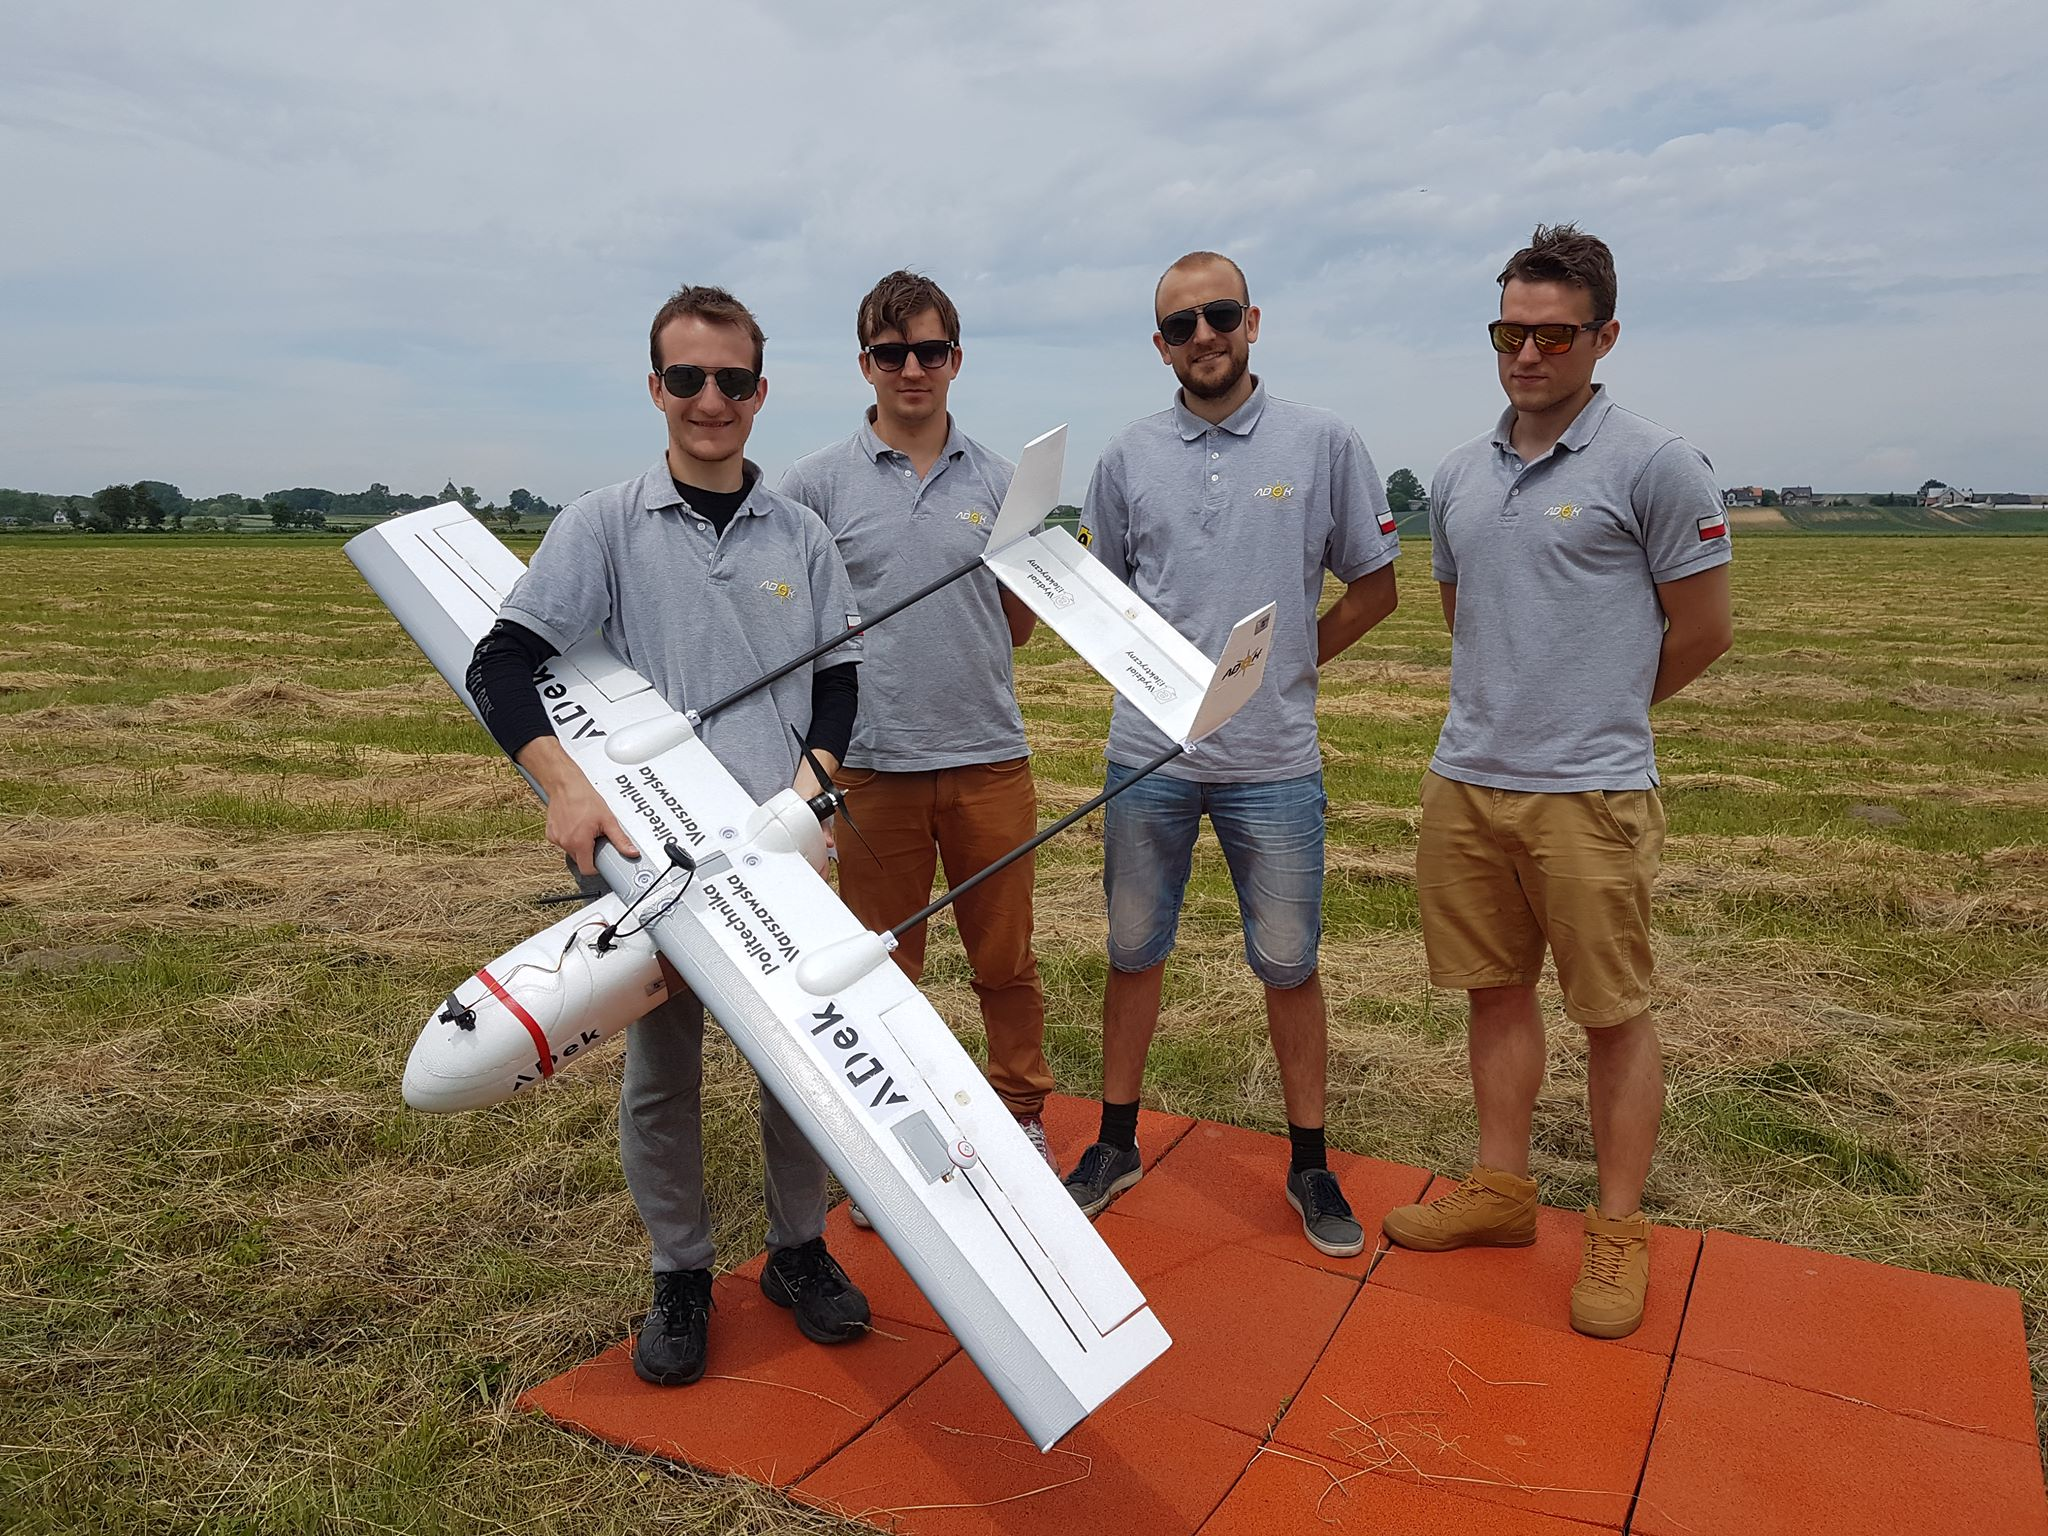
\includegraphics[width=15cm]{zalaczniki/obrazy/droniada.jpg}
    \caption{Część naszego zespołu na konkursie "Droniada", osoby które brały udział w konkursie głównym}
    \label{fig:zespoldroniada}
\end{figure}

\subsection{Wprowadzenie do zagadnienia}

Projektowany system składał się z kliku części, schemat ideowy systemu przedstawia rysunek \ref{fig:schematIdeowy}. Część pierwsza to poszkodowane w katastrofie osoby, a właściwie beacony które ratownicy medyczni wręczyli poszkodowanym osobom, beacony nadają uzgodniony sygnał reprezentujący pewien kolor, i tak kolor czerwony jest przyporządkowany do osób co do których wymagana jest natychmiastowa ewakuacja, kolorem żółtym oznaczone zostają osoby, które wymagają pilnej ewakuacji (mniejszy priorytet), kolorem zielonym osoby które chodzą o własnych siłach, natomiast kolorem czarnym zgony, osoby których ciała zostaną usunięte dopiero po zakończeniu akcji ratowania życia. Jest to tzw. system znaczników Triage \cite{triage}, rysunek \ref{fig:triage} przedstawia przykładowy, papierowy, używany przez ratowników znacznik systemu Triage. Moim zadaniem jest próba udowodnienia że taki papierowy znacznik można zamienić na beacon, który nadając dookolnie zakodowany sygnał pomoże ratownikom w akcji ratunkowej.

\begin{figure}[!th]
    \centering
    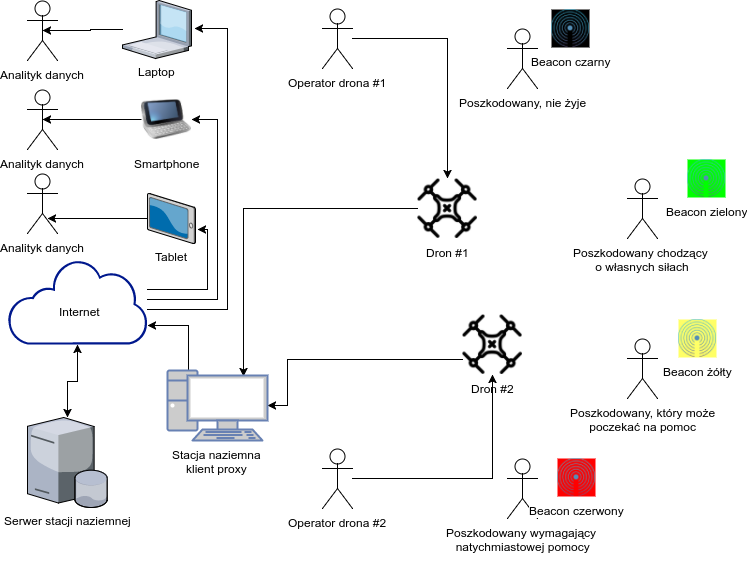
\includegraphics[width=15cm]{zalaczniki/obrazy/schemat_ideowy.png}
    \caption{Schemat ideowy systemu, widać na nim wszystkie elementy systemu, począwszy od poszkodowanych, przez drony i ich operatorów, a skończywszy na wszystkich elementach stacji naziemnej i analitykach zebranych danych}
    \label{fig:schematIdeowy}
\end{figure}

\begin{figure}[!th]
    \centering
    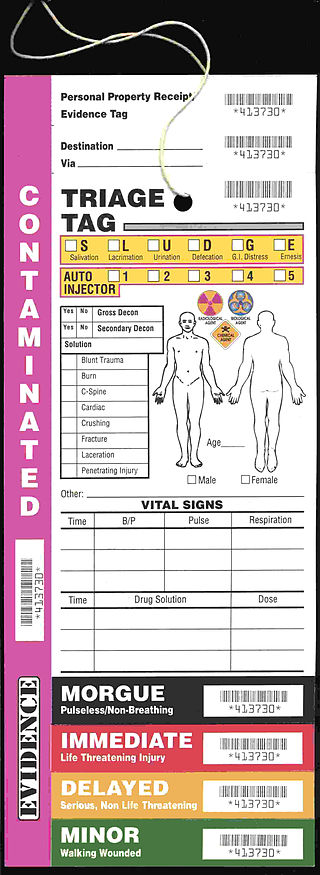
\includegraphics[width=5cm]{zalaczniki/obrazy/triage_tag.jpg}
    \caption{Typowy znacznik systemu Triage, używany w akcjach ratowniczych \cite{triage}}
    \label{fig:triage}
\end{figure}

Kolejnym komponentem systemu był statek powietrzny, który miał za zadanie zbieranie nadawanych przez beacony sygnałów i umiejscawianie ich na płaszczyźnie mapy. Taki statek musiał zostać wyposażony w odbiornik bluetooth, w wersji co najmniej 4.0 i odpowiednie oprogramowanie zbierające sygnały.

Ostatnim elementem systemu był system naziemny (ang. Ground Station). System ten zbierał zlokalizowane przez statek powietrzny sygnały i wyświetlał je na mapie, dodatkowo aproksymując pozycję realną beaconów na mapie. System ten składał się z kilku komponentów w architekturze klient-serwer.

Ogólny diagram BPMN mojego rozwiązania przedstawia rysunek \ref{fig:diagramogolny}. Na pierwszym torze widzimy beacona, na drugim statek powietrzny, na ostatnich trzech przedstawiona jest stacja naziemna. Stacja naziemna mogła być dowolnie dzielona na fizyczne maszyny, w moim przypadku połączona była stacja naziemna z klientem proxy i z klientem odbiorczym, stacja naziemna z oprogramowaniem serwera była na innej maszynie fizycznej. W kolejnych rozdziałach będę przybliżał kolejne komponenty systemu.

\begin{figure}[!th]
    \centering
    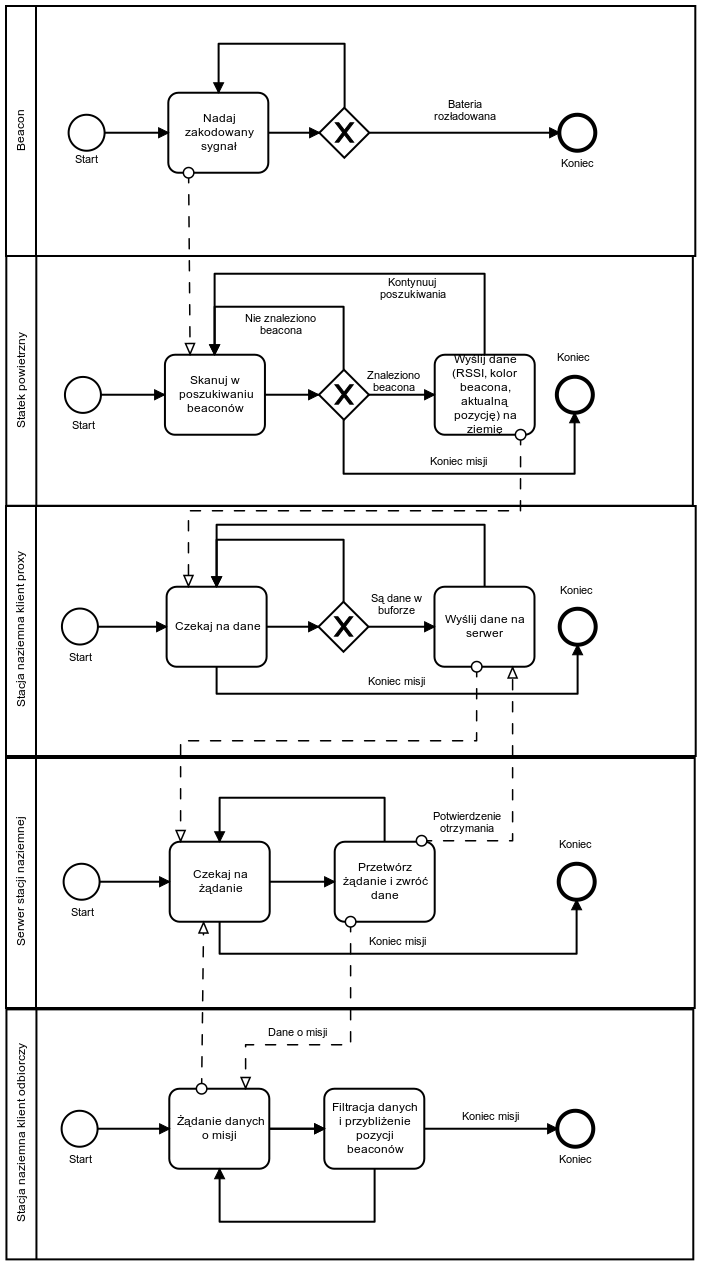
\includegraphics[width=12.8cm]{zalaczniki/obrazy/diagram_ogolny.png}
    \caption{Ogólny diagram BPMN przepływu danych w systemie}
    \label{fig:diagramogolny}
\end{figure}

\section{Internet rzeczy}

\subsection{Koncepcja pomysłu internetu rzeczy}

Internet rzeczy (ang. \textit{Internet of Things - IoT}) to idea która zakłada że wszystko można podłączyć do sieci internet \cite{iot}, wszystko to znaczy pojazd, budynek i inne rzeczy wyposażone w elektroniczny system wbudowany z sensorami, aktorami oraz interfejs sieciowy, dzięki czemu możliwa jest wymiana danych. 

Podstawowym celem idei internetu rzeczy jest stworzenie inteligentnych rzeczy, budynków, miast itp. Takie inteligentne rzeczy połączone w sieci, mogą dać ludzkości możliwość nieustannego monitorowania zmieniających się warunków i przystosowywania tych inteligentnych rzeczy do wymagań użytkowników. Dla przykładu sieć czujników, które zbierają dane pogodowe takie jak temperatura, ciśnienie, wysokość poziomu rzek itp. mogłaby w czasie rzeczywistym wykrywać anomalie i sama na nie reagować. Taka szybka reakcja na zagrożenie, znacząco zwiększa szanse na uratowanie ludzkiego życia i zmniejsza straty materialne.

\subsection{Infrastruktura, sprzęt i BLE \cite{infrastrukturaiot}}

Warstwa odpowiedzialna za zbieranie danych ze świata rzeczywistego, wyposażona jest przede wszystkim w sensory i elektroniczne identyfikatory. Sensory już od bardzo dawna używane są w przemyśle samochodowym, służbie zdrowia, zakładach produkcyjnych czy przemyśle kosmicznym, są coraz tańsze i mniejsze, dzięki temu mogą być dodawane jako standardowe wyposażenie do dowolnych urządzeń. Większość współczesnych telefonów jest wyposażona w akcelerometr, magnetometr, żyroskop, czujnik zbliżeniowy, czujnik oświetlenia, a nawet czujnik wilgotności, czy barometr. Projekt CeNSE (ang. Central Nervous System of the Earth) ma na celu rozwój technologii w taki sposób, aby umożliwić oczujnikowanie całej naszej planety, tworząc swoisty układ nerwowy \cite{cense}.

Bardzo ważną warstwą sieci internetu rzeczy, jest warstwa transportowa. Warstwa transportowa łączy wszystkie sensory i aktory do sieci internet. Prowadzenie sieci kablowej jest bardzo drogie i czasochłonne, dlatego urządzenia implementujące ideę internetu rzeczy najczęściej wykorzystują różnorakie technologie bezprzewodowe, na przykład:

\begin{itemize}
	\item{Sieci komórkowe 2G, 3G, 4G - wymagają one doposarzenia urządzenia w kartę SIM}
	\item{WiFi - sieci małego zasięgu, dla zapewnienia dostępu do internetu wymagany jest punkt dostępowy}
	\item{Bluetooth - protokół dedykowany sieciom osobistym, stosunkowo duże prędkości przesyłu}
	\item{ZigBee - niska przepustowość, energooszczędność, spory zasięg w porównaniu z dwiema wyżej wymienionymi pozycjami}
	\item{Z-Wave - protokół dla domowej automatyki, wykorzystuje radio małej mocy}
\end{itemize}

Urządzeniem które powstało specjalnie dla internetu rzeczy jest tzw. beacon, jest to urządzenie małej mocy które, w z góry określonych interwałach czasowych, nadaje dookolnie ramki danych przy wykorzystaniu bluetooth. Ważne jest że beacon ma zaimplementowany bluetooth w wersji 4.0 (lub wyższej) potocznie nazywany BLE (ang. \textit{Bluetooth Low Energy}). Ramki te, mogą odbierać urządzenia znajdujące się w pobliżu beacona, zasięg typowego beacona to około $100 m$, na podstawie odebranego sygnału urządzenia mogę podejmować akcje. Ważnym parametrem sygnału nadawanego przez beacony, w naszym przypadku było tzw. RSSI, jest to po prostu miara siły sygnału odebranego przez urządzenie odbiorcze. Im większy parametr RSSI tym mocniejszy sygnał, dzięki temu można, z dość dużym błędem niestety, powiedzieć jak daleko znajdujemy się od nadajnika sygnału.

\subsection{Komponenty IoT wykorzystane w tworzonym systemie}

W tworzonym systemie wykorzystaliśmy beacony, jako urządzenia którymi oznaczane były osoby poszkodowane. Beacony to małe nadajniki sygnału radiowego, które najczęściej są używane do wysyłania danych na nasze telefony, w ogólności odbiornikiem może być dowolne urządzenie wyposażone w bluetooth w wersji 4.0 lub większej. Beacon często nazywany jest latarnią, działa on bowiem jako taka latarnia, zazwyczaj jest umieszczony w jednym, konkretnym miejscu, gdy wejdziemy w zasięg nadawanego przez niego sygnału możemy odbierać dane przez niego nadawane i na nie reagować. Beacony konkursowe nadawały dane przy wykorzystaniu protokołu iBeacon\cite{ibeacon}, stworzonego przez firmę Apple, innym równie popularnym protokołem jest Eddystone \cite{eddystone}, jednak ja w tej pracy skupiłem się na protokole iBeacon. To co nas najbardziej interesowało to bajty z danymi Major i Minor, oznaczającymi kolejno kolor i numer beacona według specyfikacji w tabeli \ref{tab:minormajor}.

\begin{tablica}
    {Kodowanie kolorów na dane Minor i Major}
    {Kodowanie kolorów na dane Minor i Major}
    {
    \begin{tabular}{|c|c|p{10cm}|} \hline
	    \textbf{Major.Minor} & \textbf{Kolor} & \textbf{Znaczenie} \\ \hline
	    \multirow{2}{*}{1.1} & \multirow{2}{1.65cm}{Czarny} & Katgoria BLACK, stwierdzono zgon, ciało zostanie zabrane po akcji ratunkowej. \\ \hline
	    2.1 & \multirow{2}{1.65cm}{Zielony} & \multirow{2}{10cm}{Odpowiednik kategorii GREEN, poszkodowany chodzi o własnych siłach - zdalny nadzór.} \\
	2.2 & &  \\ \hline
	    3.1 & \multirow{3}{1.65cm}{Żółty} & \multirow{3}{10cm}{Odpowiednik kategorii YELLOW, pilna ewakuacja medyczna.} \\
	3.2 & &  \\
	3.3 & &  \\ \hline
	    4.1 & \multirow{4}{1.65cm}{Czerwony} & \multirow{4}{10cm}{Odpowiednik kategorii RED, natychmiastowa ewakuacja medyczna poszkodowanego.} \\
	4.2 & &  \\
	4.3 & &  \\
	4.4 & &  \\ \hline
    \end{tabular}
    }
    \label{tab:minormajor}
\end{tablica}

Do odbioru sygnału beaconów, organizatorzy konkursu proponowali użycie gatewaya produkcji firmy kontakt.io \cite{gateway}. Problem był taki że wspomnianego gatewaya trzeba było zintegrować z komputerem pokładowym bezzałogowca, co wydawało się być zadaniem trudnym, ze względu na to że gateway był wyposażony w interfejsy głównie bezprzewodowe, co mijało się z celem przy kilkucentymetrowych odległościach. Postanowiłem więc użyć do tego celu komputera Raspberry Pi w wersji 3 model B \ref{fig:raspberrypi3} \cite{raspberrypimodelscomparison}, który to wspiera bluetooth 4.1, jest stosunkowo małych rozmiarów ($56,5 mm$ x $85,6 mm$ x $17 mm$), niewielkiej masy ($45g$), dodatkowo jest dość tani, wszystkie te cechy idealnie pasują do urządzenia, które można podłączyć do bezzałogowego statku powietrznego. Na Raspberry Pi zainstalowałem system RTAndroid\cite{rtandroid}, tak żeby możliwe było skorzystanie z API ułatwiającego komunikację pomiędzy beaconami i odbiornikami, utrzymywanego przez firmę kontakt.io, dzięki temu API pisanie aplikacji odbierającej dane było o wiele prostsze.

\begin{figure}[!th]
    \centering
    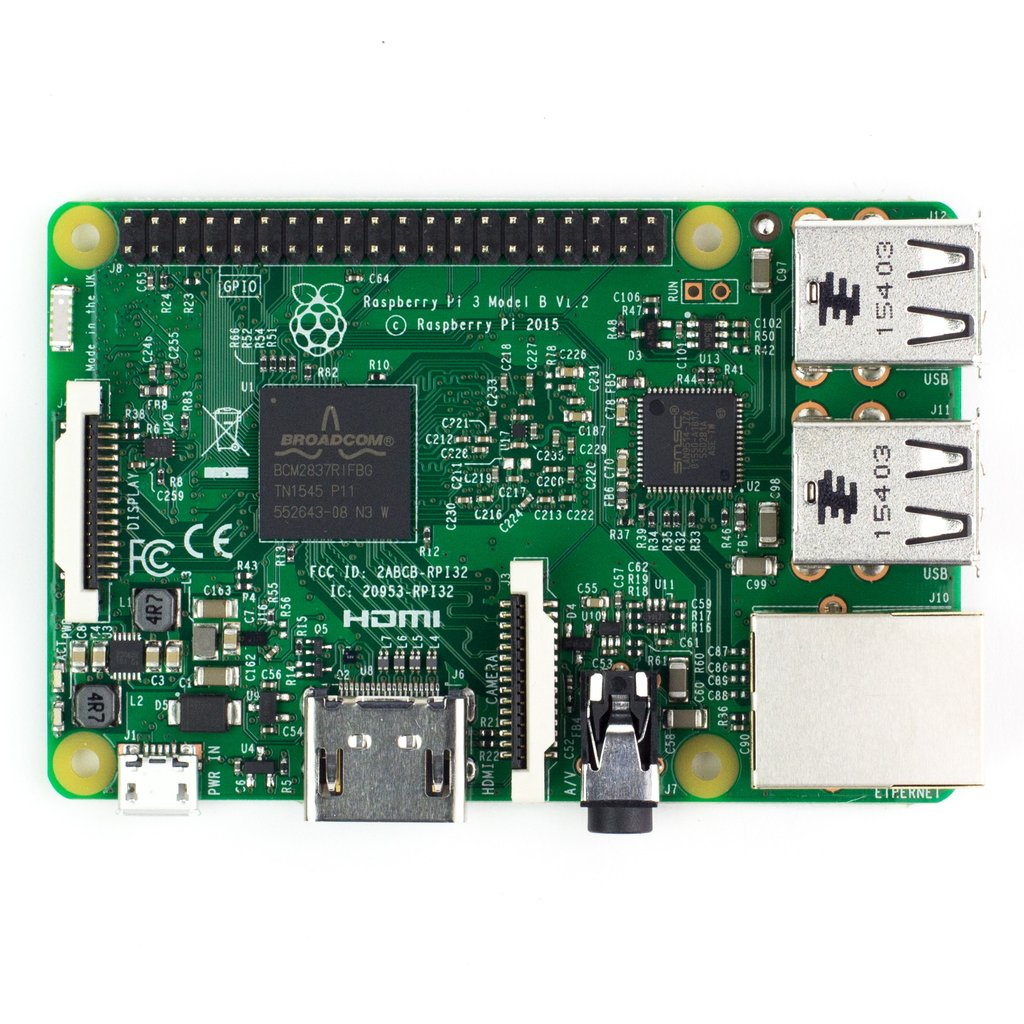
\includegraphics[width=15cm]{zalaczniki/obrazy/raspberrypi3.jpg}
    \caption{Komputer Raspberry Pi 3 Model B, użyty w moim projekcie w charakterze odbiornika bluetooth danych z beaconów}
    \label{fig:raspberrypi3}
\end{figure}

\section{Bezzałogowe statki powietrzne}

\subsection{Czym są UAV}

Bezzałogowe statki powietrzne, UAV (ang. \textit{Unmanned Aerial Vehicle}) potocznie nazywane dronami to statki powietrzne, które nie wymagają do lotu załogi obecnej na pokładzie, oraz nie mają możliwości zabierania pasażerów, pilotowane są zdalnie lub wykonują lot autonomiczny. Niegdyś wykorzystywane jedynie w wojsku, stały się jednym z symboli walki z terroryzmem, pionierami w tego typu konstrukcjach były Stany Zjednoczone oraz Izrael. Ostatnio drony za sprawą spadającej ceny komponentów z których są konstruowane, stały się dostępne praktycznie dla każdego, najczęstsze zastosowania dronów to fotografowanie i filmowanie z powietrza imprez masowych, wesel, promocja firm, turystyka, fotografowanie nieruchomości z powietrza, inwestycji typu droga szbkiego ruchu, most. Poza branżą zdjęciową, która w tym momencie jest głównym powodem zakupu dronów przez małe firmy usługowe, ale też osoby prywatne, drony znajdują zastosowanie w geodezji, ochronie, straży pożarnej, interesują się nimi firmy kurierskie, dostawcy jedzenia, w leśnictwo i wiele więcej. Drony posiadają możliwość zamontowania na ich pokładzie różnorodnych sensorów, gdzie masa sensora jest oczywiście ograniczeniem, ale dron do kwoty którą jest za niego w stanie zapłacić statystyczny Kowalski może unieść już pokaźnych rozmiarów sensory. Również mój projekt zakładał montaż takich dodatkowych sensorów na pokładzie statków powietrznych. Mój plan zakładał użycie trzech statków powietrznych do wykonania misji, jednym z nich był płatowiec widoczny na zdjęciu \ref{fig:skyhunter}, dwa pozostałe to czterowirnikowce, jeden komercyjny Phantom 3, drugi zbudowany przez nasz zespół od podstaw \ref{fig:dronczarny}.

\begin{figure}[!th]
    \centering
    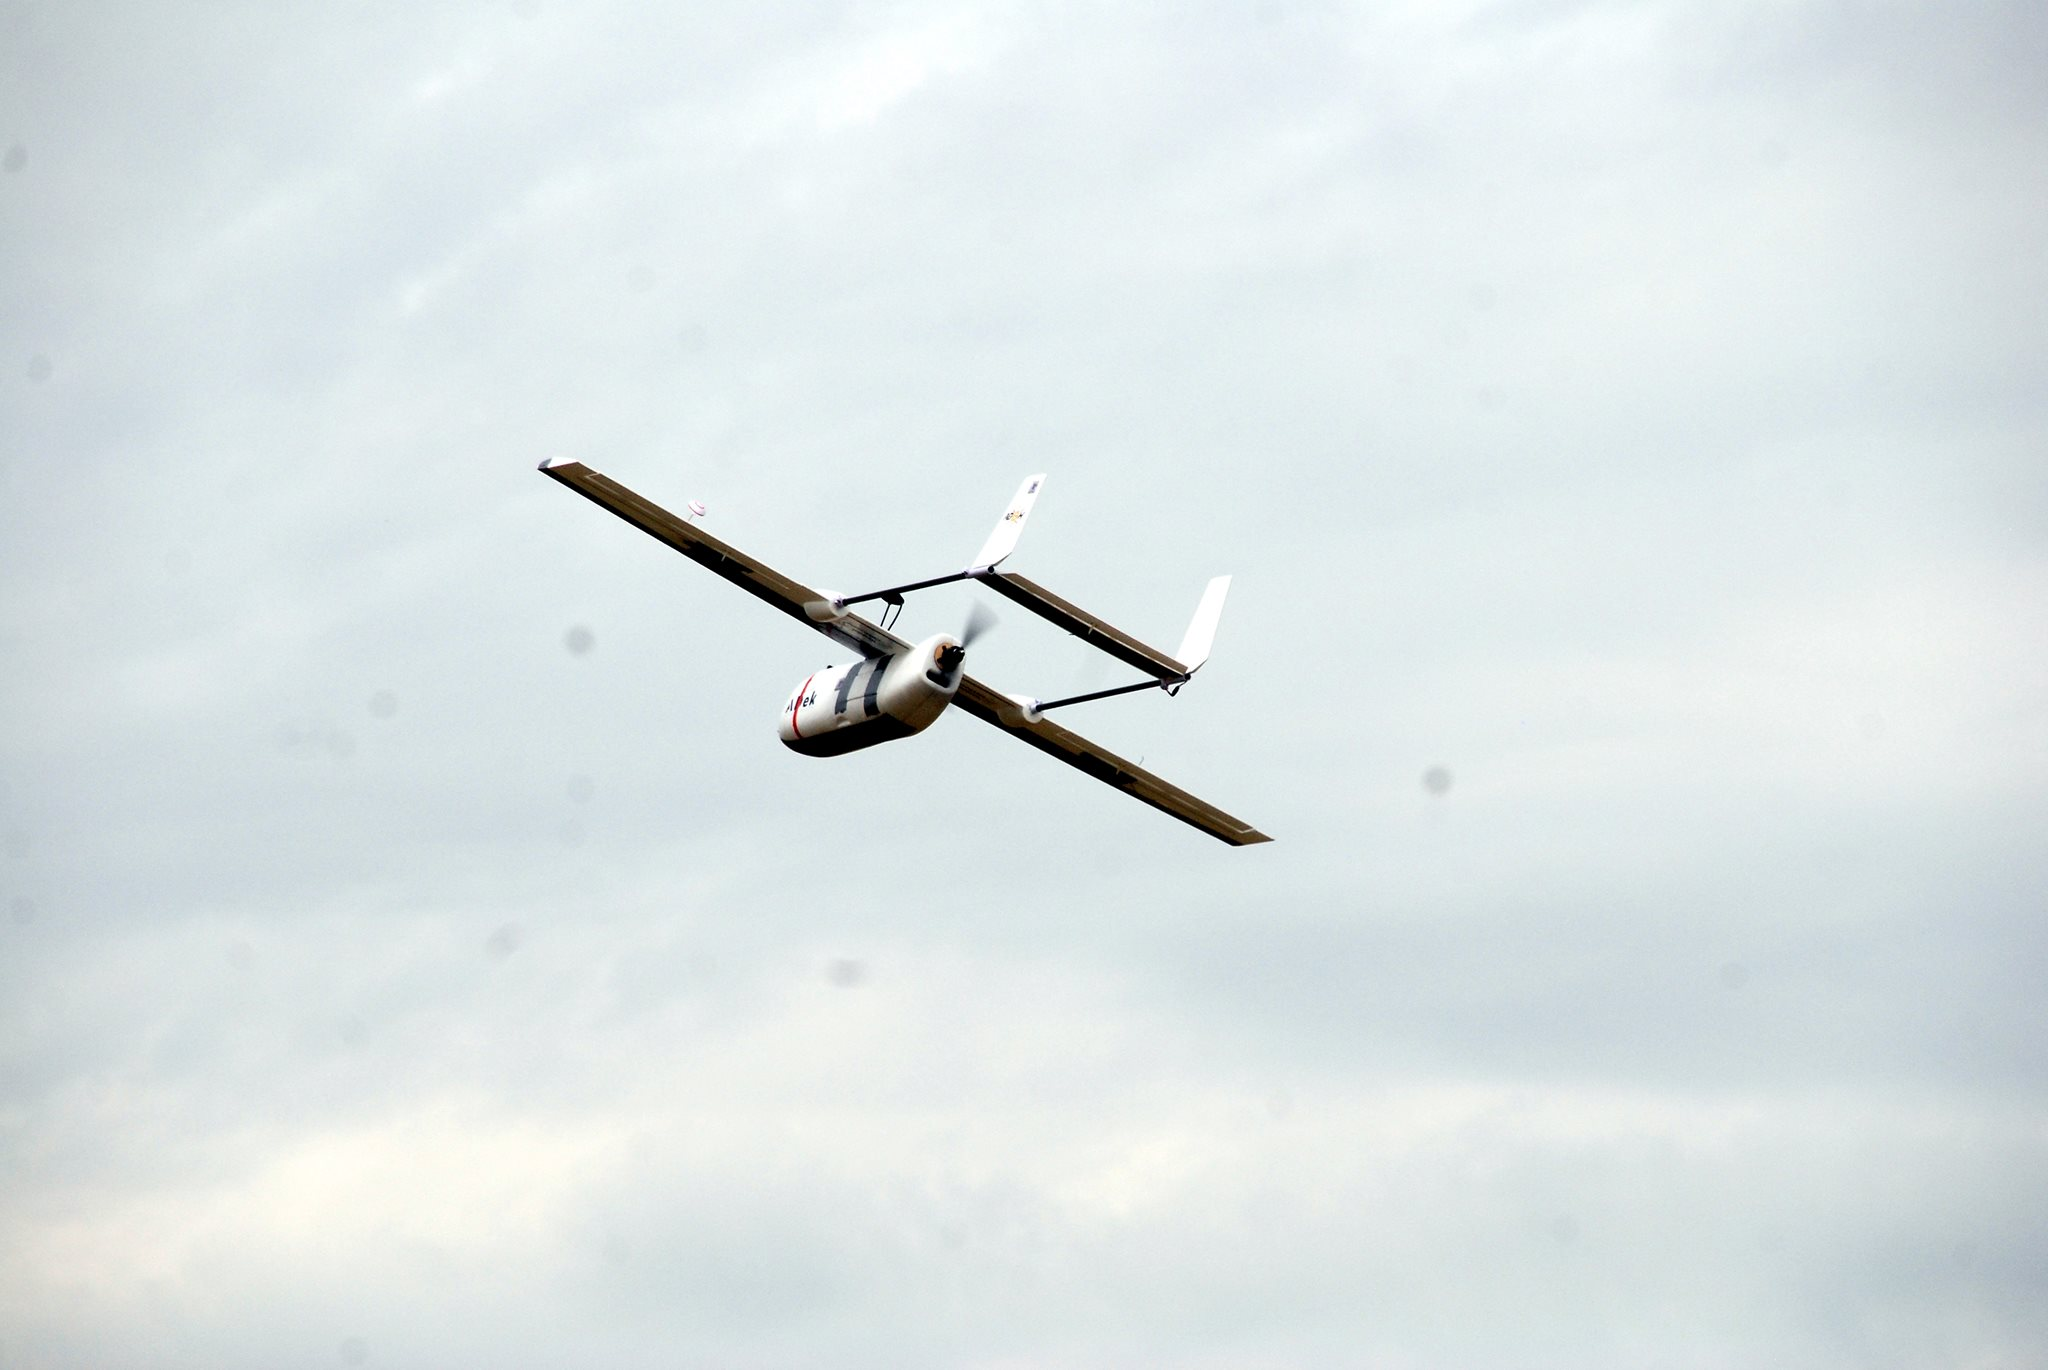
\includegraphics[width=15cm]{zalaczniki/obrazy/skyhunter.jpg}
    \caption{Nasz płatowiec, na bazie kadłuba skyhunter, podczas wykonywania misji konkursowej}
    \label{fig:skyhunter}
\end{figure}

\begin{figure}[!th]
    \centering
    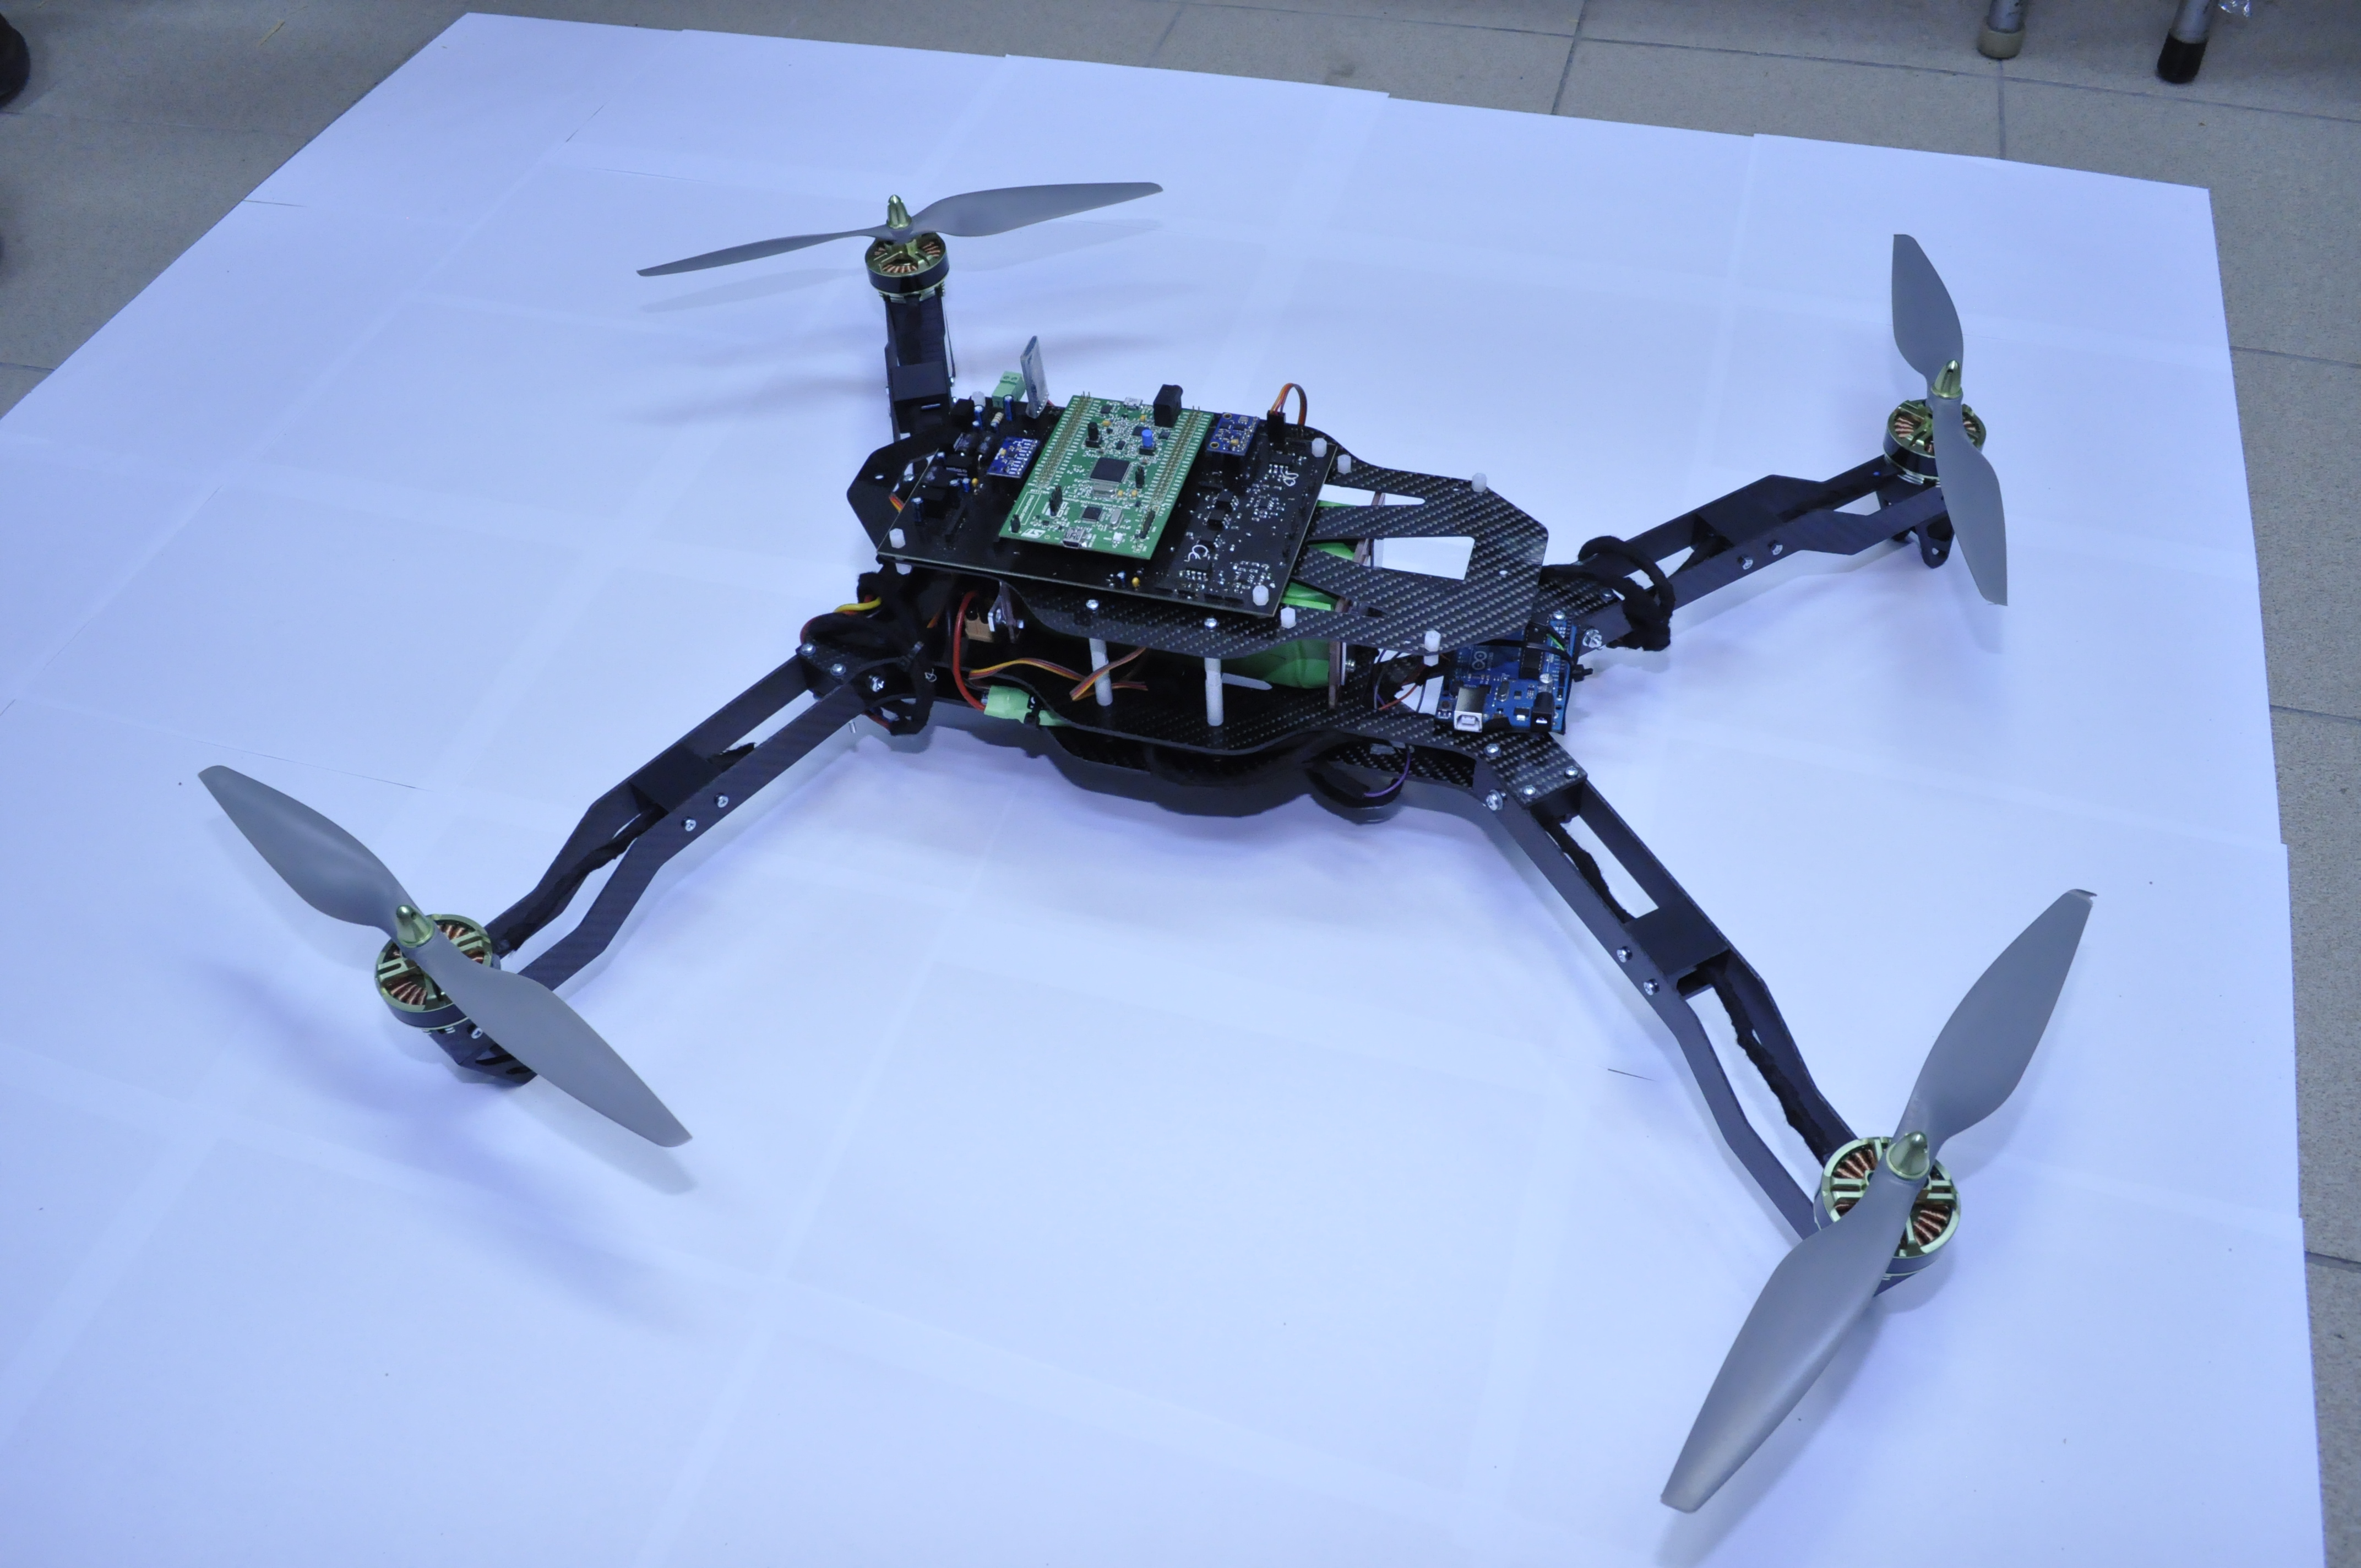
\includegraphics[width=15cm]{zalaczniki/obrazy/dron_czarny.jpg}
    \caption{Nasz czterowirnikowiec, zbudowany od podstaw, wyposażony w kontroler lotu Pixhawk}
    \label{fig:dronczarny}
\end{figure}


\subsection{Rola UAV w projektowanym systemie}

Zadaniem statków powietrznych, które wykorzystaliśmy w projekcie było znalezienie w terenie nadajników sygnału bluetooth. Teren był z góry określony i wyznaczał go wielokąt wypukły zaprezentowany na rysunku \ref{fig:teren}. Do odbioru danych, tak jak pisałem wcześniej, użyliśmy Raspberry Pi 3 Model B, po jednym komputerze do każdego statku powietrznego, mieliśmy trzy statki, więc były trzy komputery Raspberry Pi. Statki powietrzne musiały się poruszać w taki sposób, żeby po pierwsze pokryć swoim przelotem cały teren, a po drugie, zmieścić się w wyznaczonym na 30 minut oknie czasowym misji. Ważne było żeby pozycje znalezionych beaconów podać z dużą dokładnością, błąd powyżej kilku metrów oznaczał stratę punktów. Nasz plan zakładał rozpoczęcie misji płatowcem, z zaplanowaną misją, która pokrywałaby cały teren poszukiwań, do momentu znalezienia pierwszego beacona przez płatowiec, czterowirnikowce miały pozostać uziemione, w momencie nadejścia informacji o znalezieniu pierwszego beacona, pierwszy z czterowirnikowców podrywałby się i kierował w pobliże miejsca znalezienia pierwszego beacona, po zadowalającym dla nas przybliżeniu pozycji pierwszego beacona, czterowirnikowiec poruszałby się do kolejnego znalezionego beacona. Drugi czterowirnikowiec był swego rodzaju zabezpieczeniem gdyby pierwszy uległ awarii, lub gdyby pierwszy nie dawał sobie rady ze znajdowaniem kolejnych beaconów, czterowirnikowiec był sterowany manualnie przez wyszkolonego operatora, posiadającego świadectwo kwalifikacji UAVO. 

\begin{figure}[!th]
    \centering
    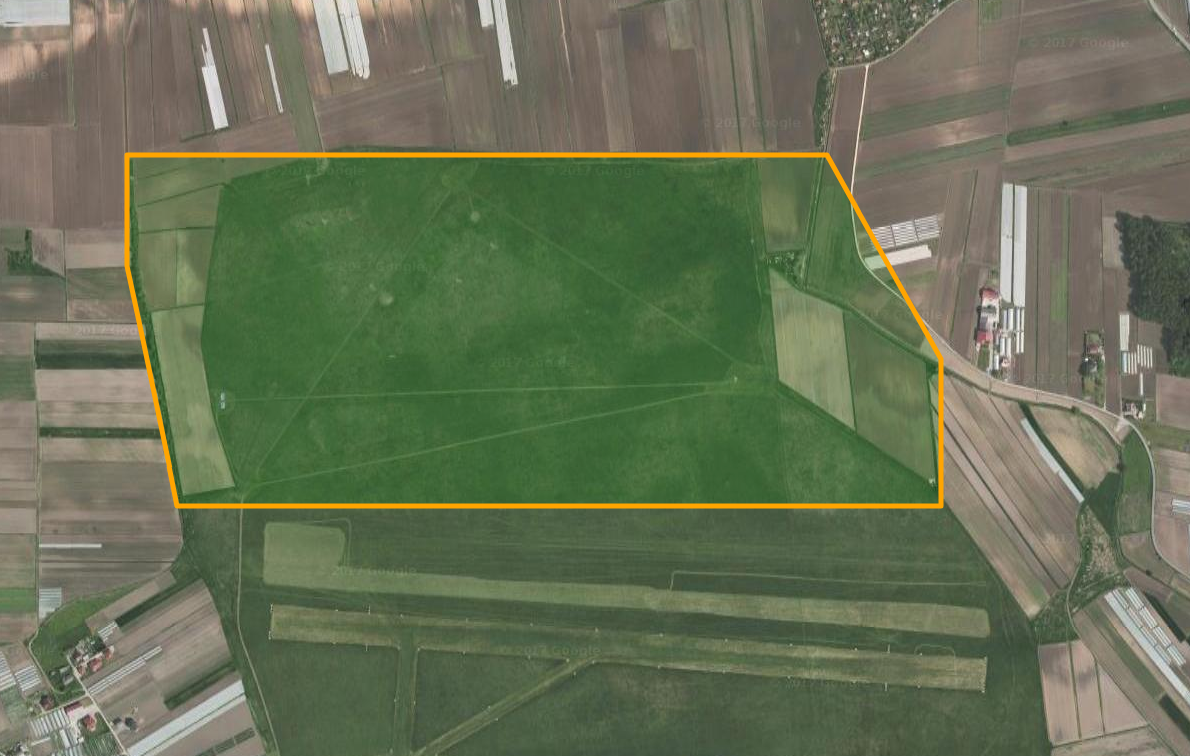
\includegraphics[width=15cm]{zalaczniki/obrazy/teren.png}
    \caption{Mapa terenu w obrębie którego mogły znajdować się beacony konkursowe, pomarańczową linią wyznaczona jest granica zewnętrzna terenu}
    \label{fig:teren}
\end{figure}

\subsection{Misja autonomiczna}

Jednym z kryteriów oceny stosowanym przez jury konkursowe, było wykonanie misji w trybie autonomicznym, to znaczy że statkami powinien sterować program komputerowy, nie człowiek. Planowanie takiej misji nie jest większym problemem, jako że stosowany przez nas kontroler lotu, Pixhawk, miał możliwość zaprogramowania mu takiej właśnie misji, planowanie misji polega na podaniu programowi punktu startu, punktu końca, oraz punktów pośrednich z wysokościami barometrycznymi, czyli wysokościami nad poziomem gruntu, na jakich ma się odbywać misja. Przykład takiej misji znajduje się na rysunku \ref{fig:misja}. My wykonywaliśmy misję w trybie częściowo autonomicznym a częściowo manualnym, płatowiec miał wgraną misję, natomiast czterowirnikowce były sterowane przez operatorów. Początkowo były plany wykonania całej misji autonomiczne, byłoby to możliwe przy wykorzystaniu narzędzia dronekit \cite{dronekit}, które to udostępnia wygodny interfejs programistyczny ułatwiający sterowanie statkami powietrznymi. Wymagałoby to jednak ode mnie napisania programu, który w odpowiedzi na znalezienie beacona przez płatowiec, wysyłałby w odpowiednie miejsce czterowirnikowiec w celu dokładniejszego zbadania pozycji beacona. Było to możliwe, ale bardzo trudne, ponieważ i tak miałem sporo pracy z innymi komponentami systemu, porzuciłem tą część projektu na samym początku. Program taki wymagałby ponadprzeciętnej obsługi sytuacji wyjątkowych, które przy takich misjach pojawiają się bardzo często (mocniejszy podmuch wiatru, przeszkoda statyczna na przykład drzewo, przeszkoda dynamiczna na przykład człowiek lub ptak) a to z kolei wymagałoby setek godzin testów i dodatkowego oprzyrządowania statku powietrznego (czujniki zbliżeniowe, zwiększenie widoczności poprzez dodatkowe lampki i ewentualne sygnały dźwiękowe w celu ostrzeżenia ludzi i odstraszenia ptaków). W rezultacie takiego programu sterującego czterowirnikowcem, nie otrzymalibyśmy niestety niczego lepszego niż jest nam w stanie zapewnić operator, żeby program przerósł operatora w tej kwestii potrzebne byłoby tysiące godzin testów, których nie byliśmy w stanie zapewnić.

\begin{figure}[!th]
    \centering
    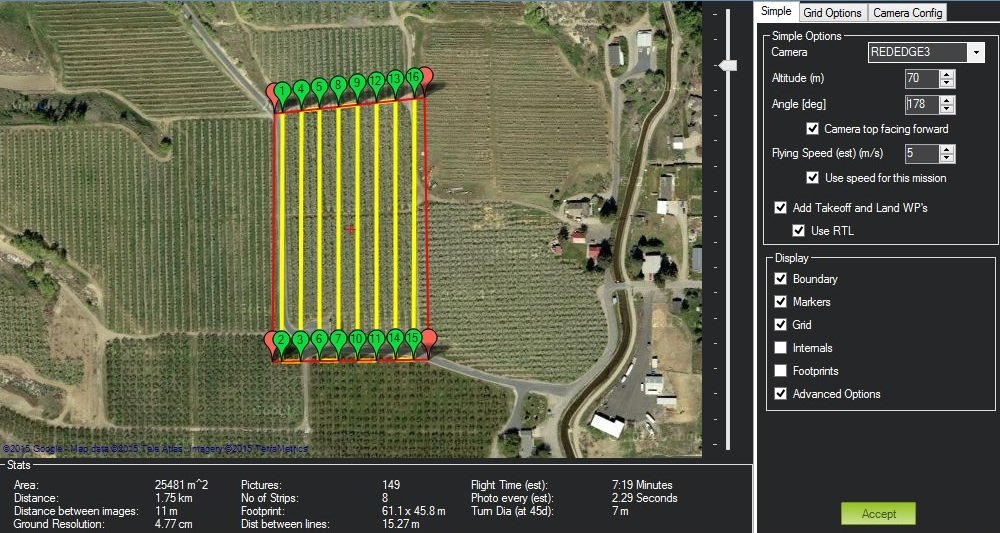
\includegraphics[width=15cm]{zalaczniki/obrazy/misja.jpg}
    \caption{Przykład misji autonomicznej w programie Mission Planner}
    \label{fig:misja}
\end{figure}

\subsection{Bezpieczeństwo stosowania UAV w misji ratunkowej}
Może się niestety tak zdarzyć że w misji ratunkowej ucierpi sam ratownik, albo jego sprzęt, mieliśmy przykład takiego incydentu podczas samego konkursu, gdzie jednej z drużyn zapaliła się bateria zainstalowana w statku powietrznym, przez co statek stanął w ogniu, sytuację przedstawiają zdjęcia \ref{fig:ploniedron1} oraz \ref{fig:ploniedron2}.

\begin{figure}[!th]
    \centering
    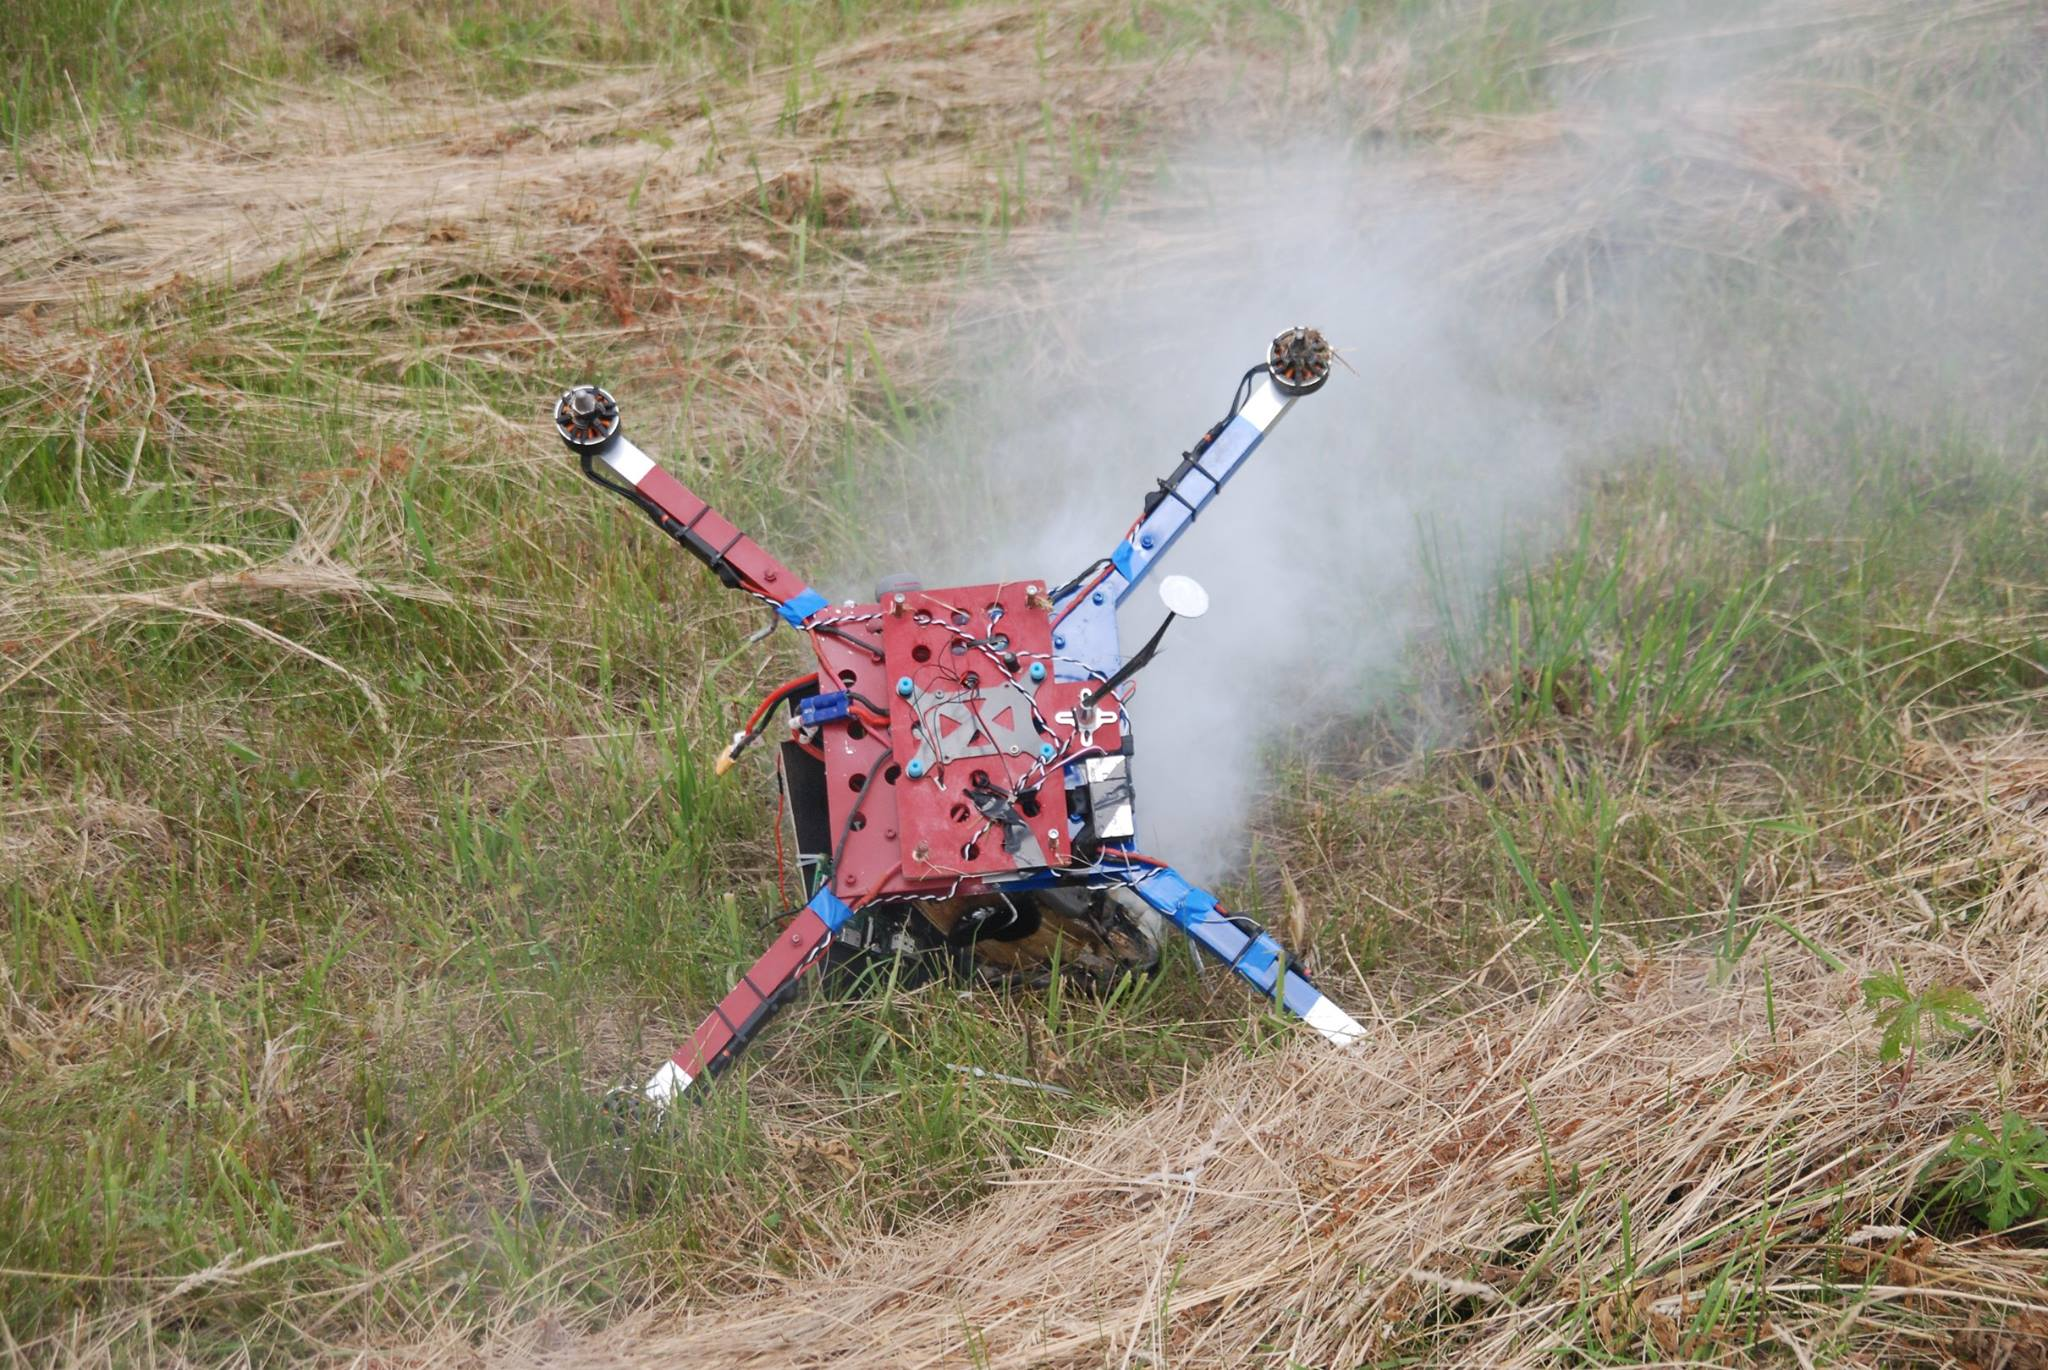
\includegraphics[width=15cm]{zalaczniki/obrazy/ploniedron1.jpg}
    \caption{Dron jednej z drużyn spłonął na zawodach}
    \label{fig:ploniedron1}
\end{figure}

\begin{figure}[!th]
    \centering
    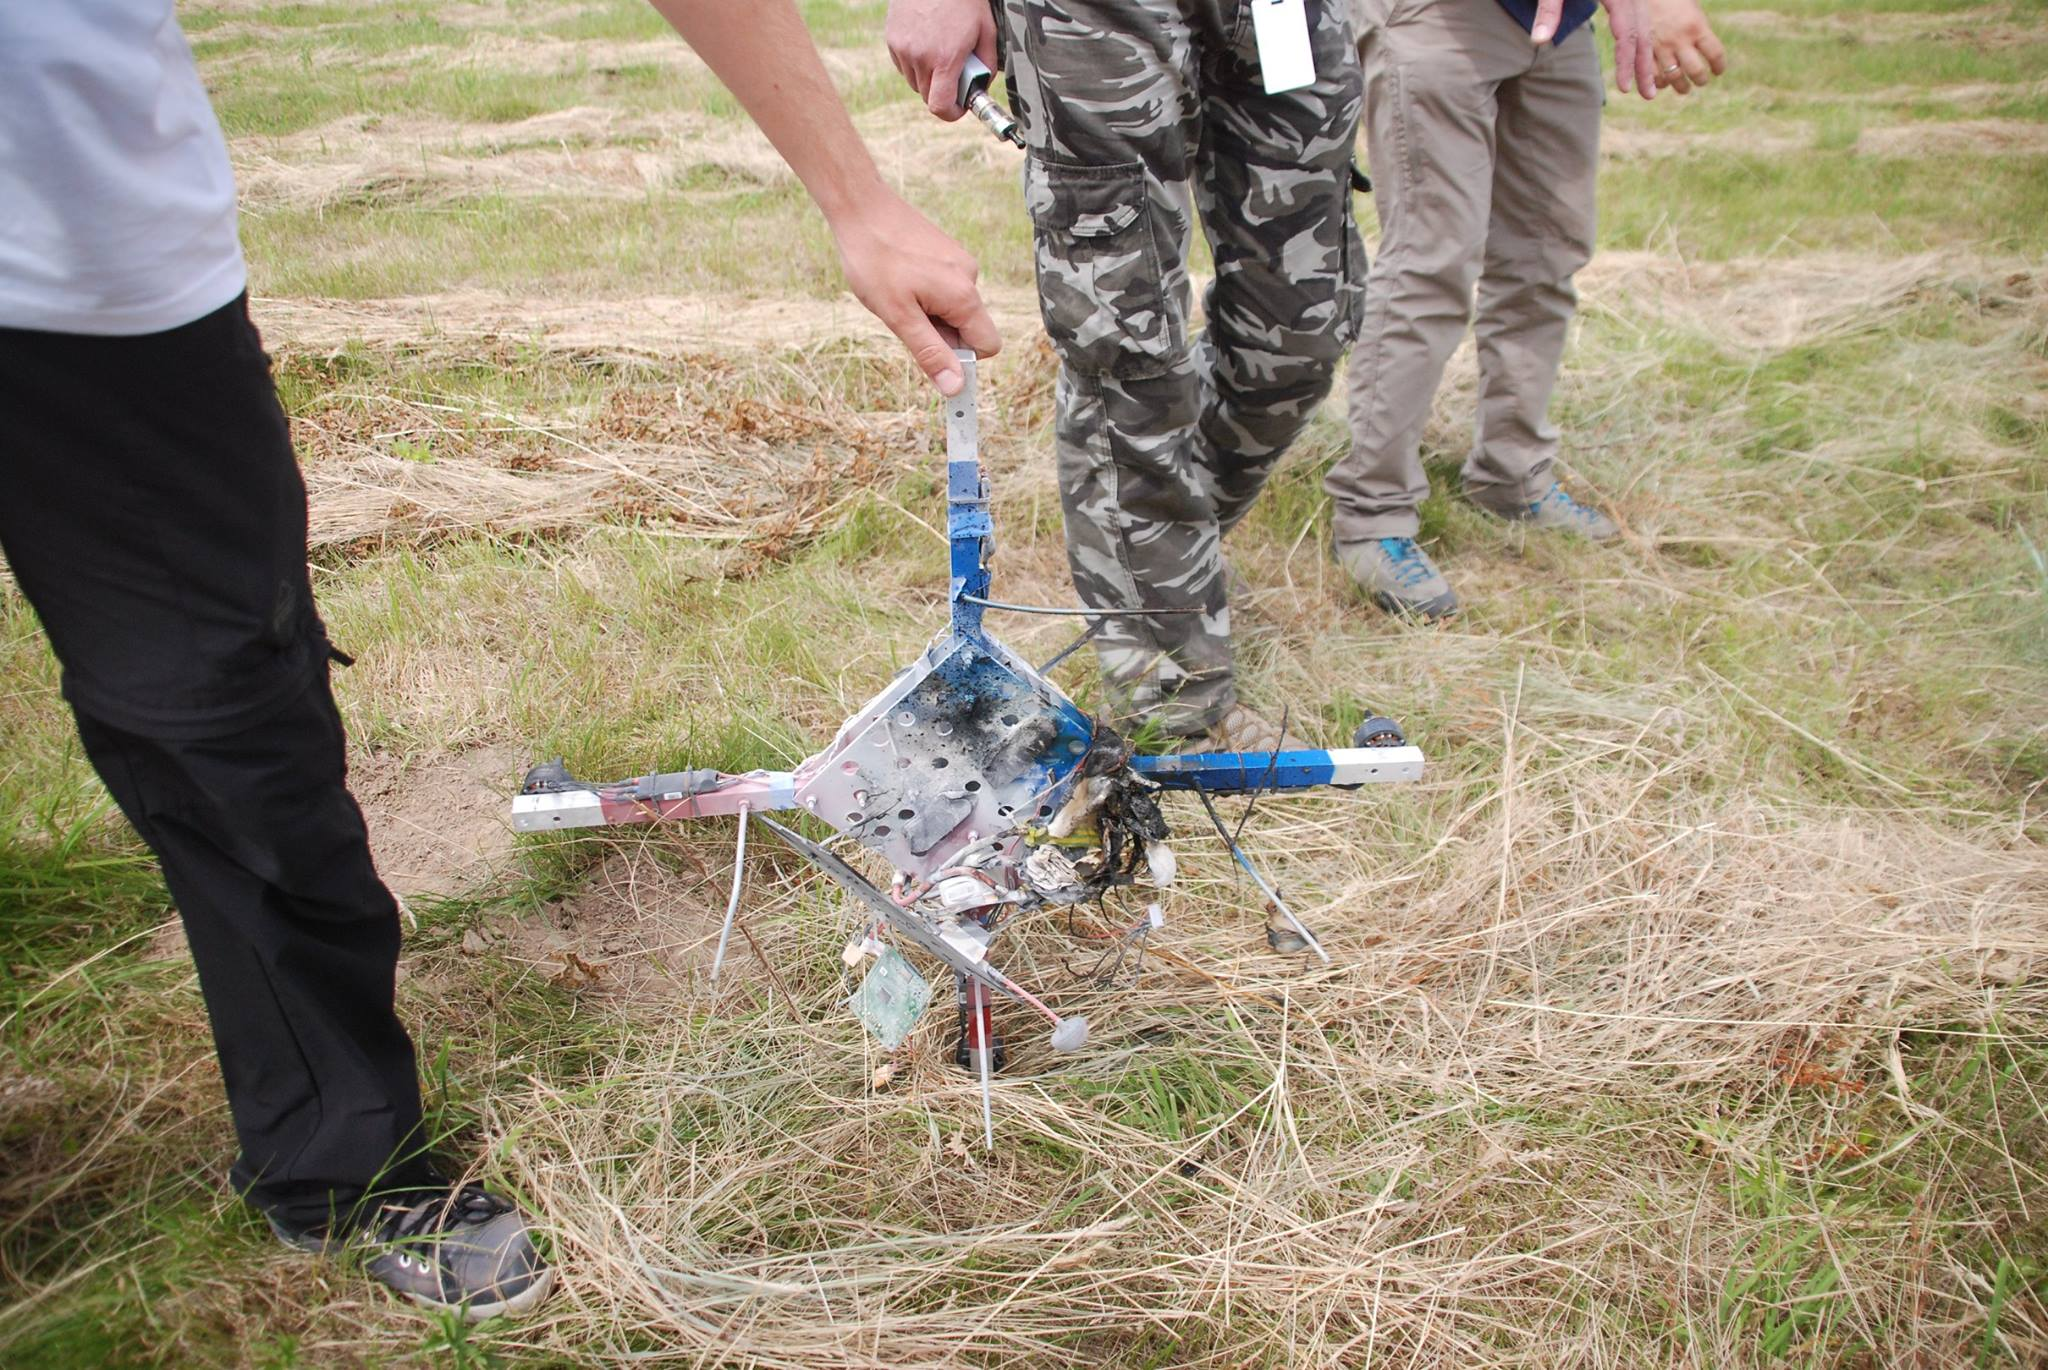
\includegraphics[width=15cm]{zalaczniki/obrazy/ploniedron2.jpg}
    \caption{To co zostało z drona po pożarze baterii}
    \label{fig:ploniedron2}
\end{figure}

Dużą wagę trzeba przyłożyć do bezpieczeństwa samego systemu, po to żeby to ratownik ratował, a żeby sam nie potrzebował pomocy. Rynek dronowy to stosunkowo nowa dziedzina i jest jeszcze dużo do zrobienia jeżeli chodzi o bezpieczeństwo, które często odkładane jest na dalszy plan, a w konsekwencji w ogóle pomijane przy projektowaniu systemów. Należy zadbać o to żeby operatorzy dronów byli dobrze widoczni, na przykład powinni mieć na sobie kamizelki w jaakrawym kolorze. Sprzęt powinien być sprawdzony przed startem, przy pomocy tzw. checklisty, gdyby drużyna której spłonął dron miała taką checklistę, może nic by się nie stało. Ważne jest też żeby operator miał ważne świadectwo kwalifikacji UAVO. Ale najważniejszy jest sam system. W dronie który spłonął prawdopodobnie brakowało systemu ostrzegania przed przegrzaniem baterii, gdyby taki system zadziałał, prawdopodobnie nic by się nie stało, drużyna nie straciłaby drona, nie doszłoby do niebezpiecznej sytuacji.

\section{Koncepcja techniczna systemu}

\subsection{Schemat blokowy rozwiązania}
Na rysunku \ref{fig:schematblokowy} znajduje się schemat blokowy zaproponowanego przeze mnie rozwiązania.
\begin{figure}[!th]
    \centering
    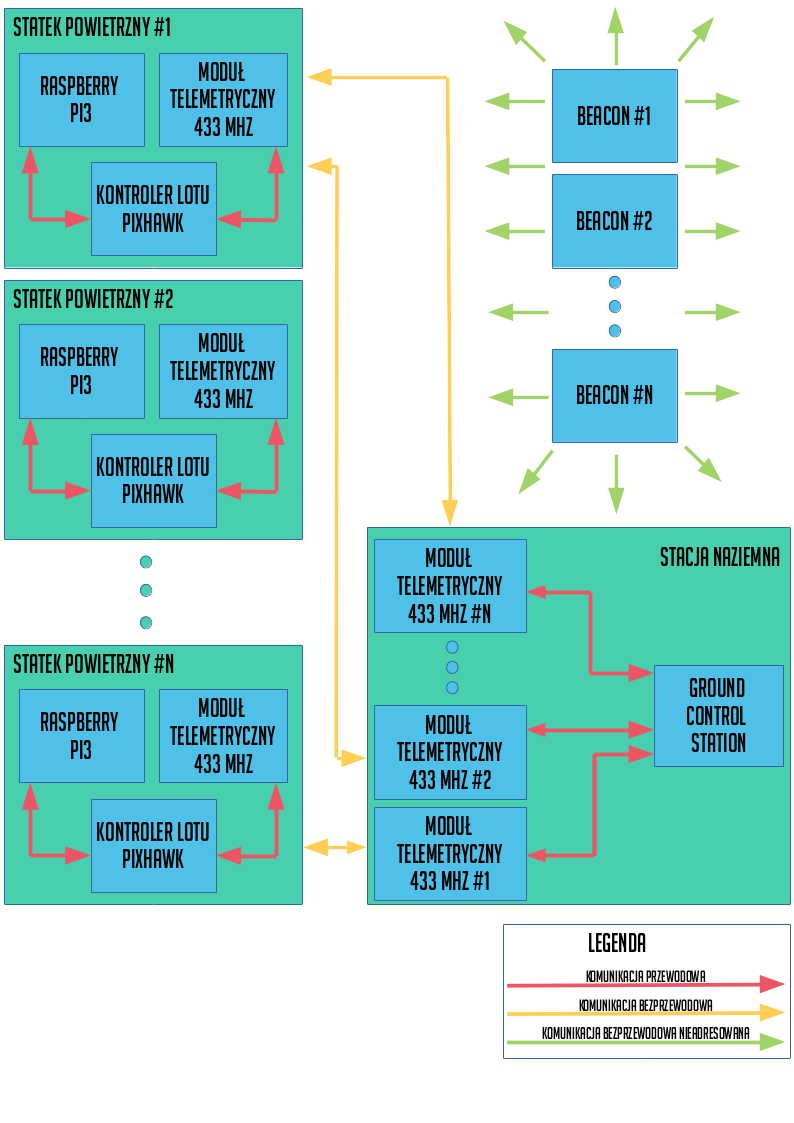
\includegraphics[width=14cm]{zalaczniki/obrazy/schemat_ogolny.png}
    \caption{Schemat blokowy systemu}
    \label{fig:schematblokowy}
\end{figure}

Stacja naziemna, to komputer z zainstalowanym oprogramowaniem i modułami telemetrycznymi, do odbierania komunikatów ze statków powietrznych. Moduły telemetryczne nie bez powodu pracują na częstotliwości $433 MHz$, jest to bowiem częstotliwość na użytkowanie której nie potrzebne jest zezwolenie, według rozporządzenia Urzędu Komunikacji Elektronicznej \cite{rozporzadzenieuke}. Stacja naziemna niekoniecznie jest miejscem przy którym siedzi operator systemu. System został zaprojektowany w architekturze klient-serwer, gdzie funkcje klientów może pełnić dowolne urządzenie, które ma dostęp sieciowy do serwera, przy czym nasz serwer znajdował się w bezpiecznym pomieszczeniu, daleko od miejsca wykonywania misji, podczas gdy my przy pomocy klientów w postaci różnych urządzeń zasilaliśmy serwer danymi, a przy pomocy innych klientów dane z serwera były pobierane i prezentowane operatorowi w wygodnej i zrozumiałej dla niego postaci, której przykład stanowi rysunek \ref{fig:klient}.

\begin{figure}[!th]
    \centering
    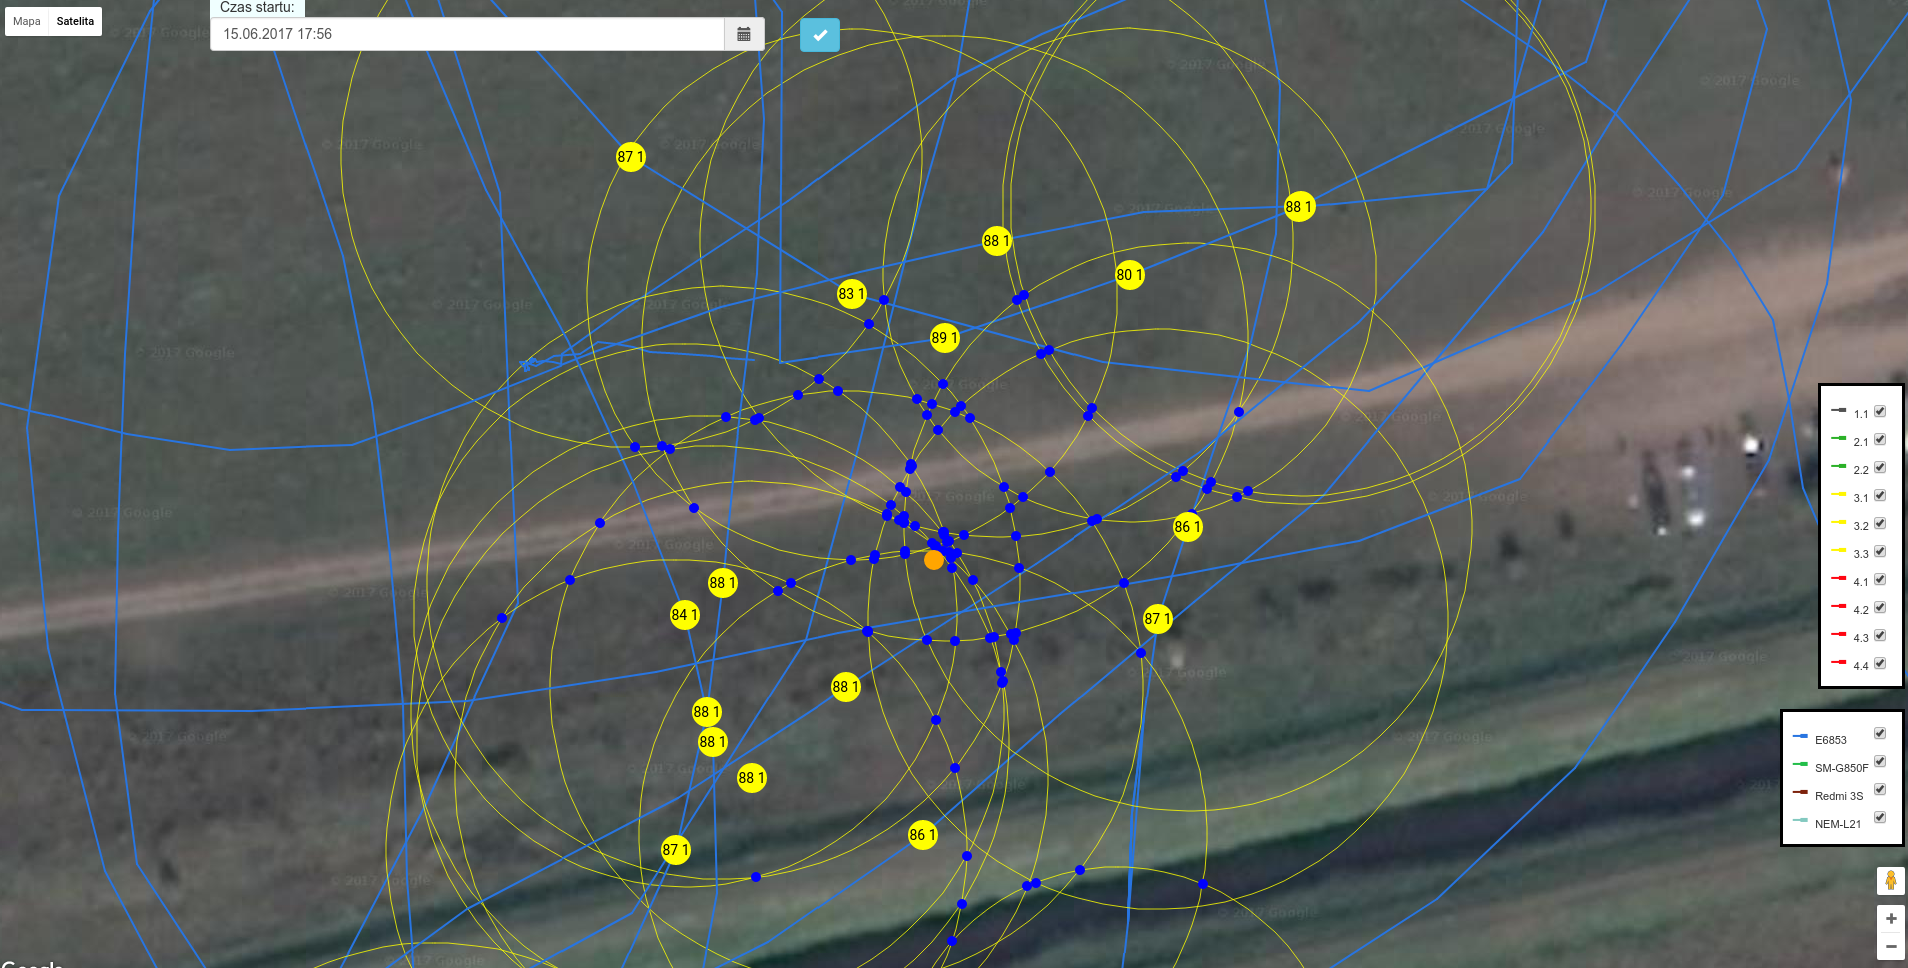
\includegraphics[width=15cm]{zalaczniki/obrazy/klient.png}
    \caption{Widok ekranu operatora systemu, w centralnym miejscu mapa z zaznaczoną trasą przelotu, próbkami znalezionego sygnału, oraz wyznaczoną aproksymacją}
    \label{fig:klient}
\end{figure}

Na rysunku widzimy dokładnie to co widzi operator systemu, zaprezentowany zrzut pochodzi z testów systemu przeprowadzanych jeszcze przed zawodami. Niebieska linia to trasa przelotu statku powietrznego, użytego do testu. Żółte kropki to próbki sygnału jakie udało się zebrać. Na kropkach pokazana jest siła sygnału (RSSI), oraz numer beacona w kolejności (w tym wypadku numer 1). Żółte okręgi wyznaczają, gdzie prawdopodobnie może znajdować się beacon (im słabszy sygnał tym większy okrąg, moja aproksymacja działa podobnie jak ta która działa w systemie GPS). Tam gdzie żółte okręgi się przecinają stawiamy granatowy punkt, ale nie zawsze, wybieramy tylko te punkty które są najbliżej prawdopodobnego rozwiązania, w końcu pomarańczowy punkt stanowi rozwiązanie aproksymacji. W przedstawionym przykładzie system pomylił się około 2 metry na południe, co mogło być wynikiem dokładności systemu GPS i małej ilości próbek sygnału w zaprezentowanym przykładzie.

Dodatkowo operator, po prawej stronie ekranu, ma możliwość włączenia lub wyłączenia ścieżek pojazdów, oraz poszczególnych beaconów, co może być przydatne w przypadku dużej ilości zebranych danych. Na górze jest też możliwość wybrania z systemu danych, od konkretnego momentu w czasie, na przykład możemy wybrać tylko punkty, które zostały utworzone dzisiaj po godzinie 14:00, opcja ta była przydatna podczas przeprowadzania testów.

Wracając do schematu blokowego, kolejnym jego elementem są statki powietrzne, ich ilości w projektowanym systemie nie ograniczało nic. W praktyce oczywiście, ograniczeniem mogłaby być przepustowość łącza jaką dysponowaliśmy, ilość operatorów potrzebnych do obsługi statków i na pewno same statki, które nie są przecież tanie. Wymaganie jakie było postawione naszym statkom powietrznym, to posiadanie kontrolera lotu pixhawk, miejsce na umieszczenie modułu Raspberry Pi 3, oraz posiadanie linku telemetrycznego $433 MHz$. Od konieczności posiadania Pixhawka poczyniliśmy jednak odstępstwo, ponieważ daliśmy możliwość pracy ze statkiem komercyjnym, jakim jest Phantom 3 \ref{fig:phantom}, nie ma on na wyposażeniu kontrolera lotu Pixhawk, a jedynie co było wymagane żeby Phantom mógł zasilać nasz system danymi, to podczepienie mu urządzenia z zainstalowaną aplikacją, urządzeniem mogło być Raspberry Pi 3, lub na przykład dowolny telefon, wyposażony w bluetooth 4.0 lub większy.

\begin{figure}[!th]
    \centering
    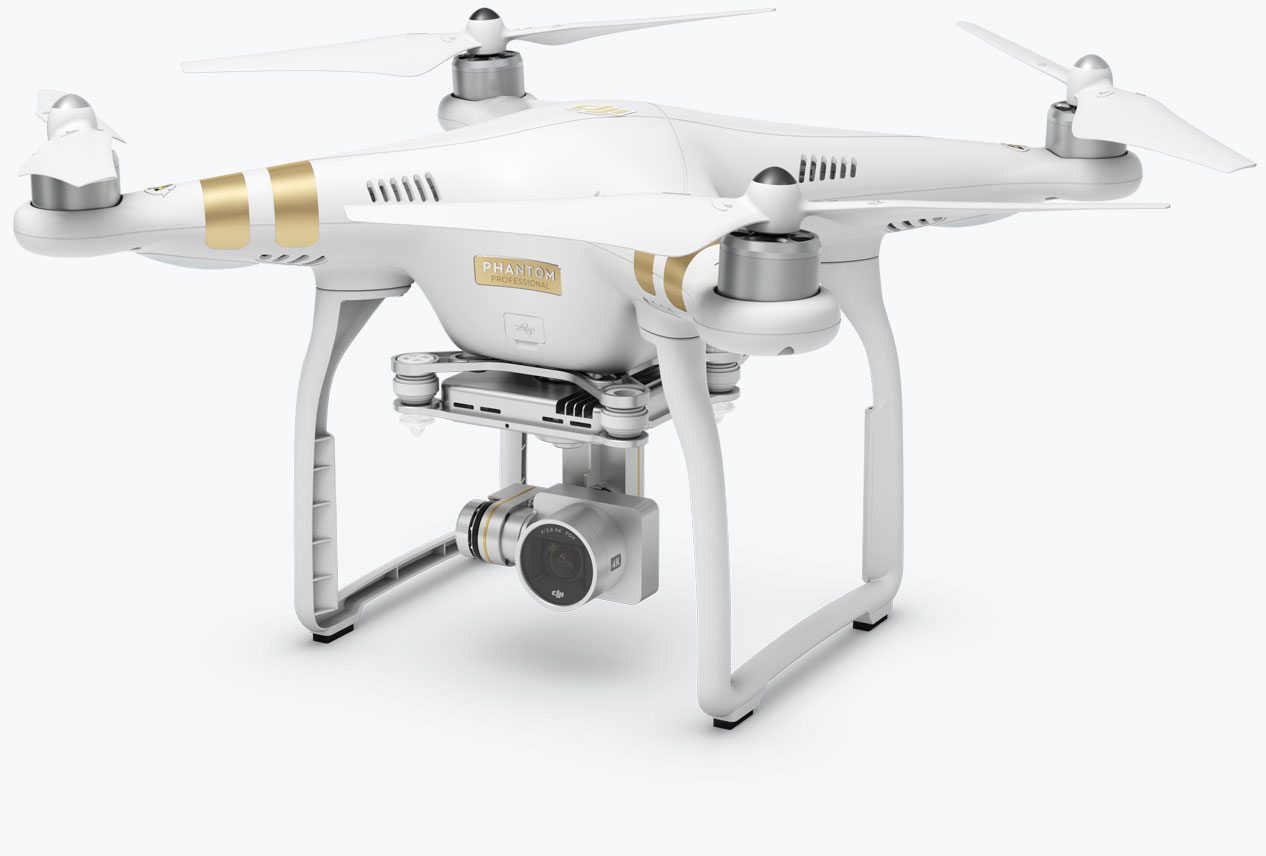
\includegraphics[width=15cm]{zalaczniki/obrazy/phantom3.jpg}
	\caption{Komercyjny dron Phantom 3, użyty przez nas w misji}
    \label{fig:phantom}
\end{figure}

Ostatnim elementem zaprezentowanym na schemacie są beacony. Są to urządzenia wyposażone w nadajnik bluetooth, który ma możliwość wysyłania dookolnych, niezaadresowanych danych. Dzięki temu że dane nie są zaadresowane, nie trzeba parować urządzeń (tak jak miało to miejsce przed pojawieniem się bluetooth 4.0). Sygnały nadawane przez wspomniane beacony byłby zbierane przez statki powietrzne, a właściwie przez aplikację zainstalowaną na Raspberry Pi 3, lub innym urządzeniu i wysyłane do stacji naziemnej.

\subsection{Algorytm pracy}

Algorytm pracy systemu jest następujący. Pierwszym krokiem jest rozmieszczenie włączonych beaconów, nadających dane w ustalonym wcześniej protokole \ref{tab:minormajor}, na jakimś z góry ustalonym obszarze. Beacony, przypominam symulują osoby które ucierpiały w katastrofie.

Kolejnym krokiem jest uruchomienie klientów, czyli urządzeń które będą sygnały zbierać, i umieszczenie ich na statkach powietrznych.

Następnie podłączamy się klientem który będzie dane odbierał, jako że moja aplikacja została napisana w technologii webowej, klientem odbiorczym mogło być dowolne urządzenie posiadające dostęp do serwera i przeglądarkę internetową, na przykład laptop.

Od tego momentu rozpoczyna się misja właściwa, statki wznoszą się w powietrze i oblatują wskazany teren, mogą to robić autonomiczne, z pomocą zaprogramowanej wcześniej przez operatora misji, lub operator sam może kierować ich ruchem, można też oczywiście stosować mieszaną taktykę, konfiguracja jest dowolna, statki są od siebie niezależne. Aplikacja zainstalowana na urządzeniu podczepionym do statku, zbiera znalezione beacony i przy pomocy linku telemetrycznego wysyła je do stacji naziemnej, która transmituje je do serwera, a z serwera dowolny klient odbiorczy może je pobrać.

Klient odbiorczy ma po swojej stronie zaimplementowany algorytm aproksymacji punktu w którym prawdopodobnie znajduje się poszukiwany beacon. Doświadczony operator systemu, empirycznie na podstawie próbek sygnałów i aproksymacji, wybiera miejsce znalezienia beacona i przekazuje je do zainteresowanych osób lub innych systemów.

Algorytm pracy został przedstawiony przy pomocy diagramu BPMN na rysunku \ref{fig:diagramogolny}

\subsection{Podłączenie wielu statków do jednego systemu}

Projekt systemu od początku skupiał się na możliwości skorzystania z wielu statków powietrznych. Zostało to umożliwione, dzięki zastosowaniu infrastruktury typu klient-serwer, klientów może być dowolnie wielu i nie muszą o sobie wiedzieć, z tego punktu widzenia nie ma problemu z wieloma statkami. Również samo przybliżanie położenia beaconów, nie jest wrażliwe na ilość statków w przestrzeni, a to dzięki temu że aproksymacja dokonywana jest już po stronie klienta odbiorczego, im więcej punktów znalezionych, nawet jeżeli punkty znalazły różne statki, tym lepiej.

Może się natomiast pojawić problem innej natury, statki będą się poruszać po z góry zdefiniowanym obszarze i jak to bywa, mogą na siebie wpaść wykonując zadanie, może być to błąd operatora, błąd aparatury sterującej, błąd w programie kontrolera, usterka sprzętowa, może to też być coś z zewnątrz, ptak, drzewo, człowiek. Możliwości jest wiele, wyeliminować wszystkich zagrożeń na pewno się nie da, ale można je ograniczyć, stosując się do przyjętych procedur, przepisów prawa lotniczego, dla UAV też już są specjalne przepisy, które regulują tą coraz szybciej rozwijającą się branżę.

Ostatnią kwestią są zakłócenia. Radia statków nie są dużych mocy, raz ze względu na ograniczenia regionalne, w Polsce obowiązuje bardzo rygorystyczne prawo, jeżeli chodzi o moce nadajników, dwa ze względu na to że im mocniejsze radio, tym więcej energii konsumuje, a na statku powietrznym nie ma chyba nic cenniejszego niż energia, trzeba ją oszczędzać. Dodatkowym problemem jest ilość urządzeń korzystająca z tych samych częstotliwości, typowe częstotliwości stosowane dla UAV znajdują się w tabeli \ref{tab:typoweCzestotliwosci}.
\begin{tablica}
    {Typowe częstotliwości stosowane dla UAV}
    {Typowe częstotliwości stosowane dla UAV}
    {
    \begin{tabular}{|c|c|} \hline
        Częstotliwość & Opis \\ \hline
        $433 MHz$  & sygnał telemetryczny w Europie \\ \hline
        $915 MHz$  & sygnał telemetryczny w USA \\ \hline
        $1,2 GHz$  & sygnał audio i wideo \\ \hline
        $2,4 GHz$  & sygnał sterujący \\ \hline
        $5,8 GHz$  & sygnał audio i wideo \\ \hline
   \end{tabular}
    }
    \label{tab:typoweCzestotliwosci}
\end{tablica}

Jeden dron często używa do komunikacji z ziemią trzech a nawet czterech i więcej pasm częstotoliwości, przykład pasm wykorzystywanych przez drona Phantom 3 znajduje się na rysunku \ref{fig:phantomczestotliwosci}.

\begin{figure}[!th]
    \centering
    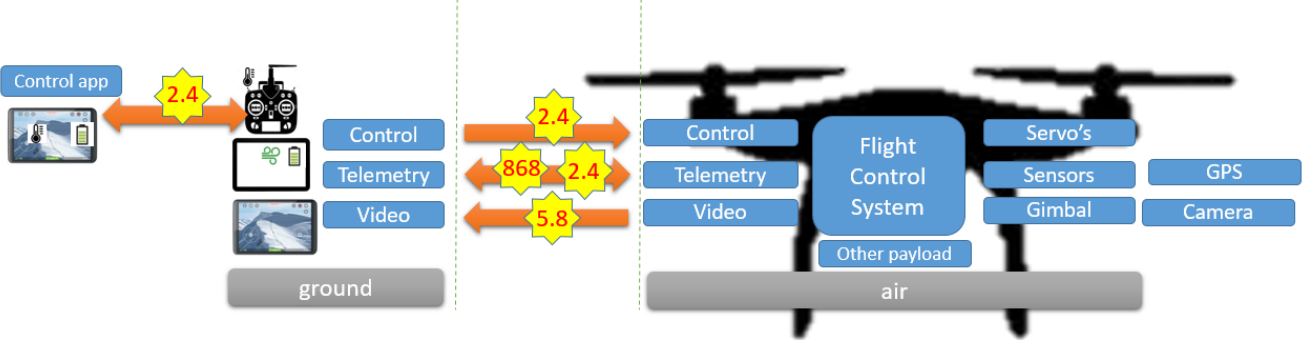
\includegraphics[width=15cm]{zalaczniki/obrazy/phantom_czestotliwosci.png}
	\caption{Częstotliwości wykorzystywane podczas lotu przez drona Phantom 3 \cite{radiointerference}}
    \label{fig:phantomczestotliwosci}
\end{figure}

Należy też pamiętać, że tych częstotliwości używają również inne technologie i rządzenia, takie jak wi-fi, bluetooth, sterowanie bram i automatyka budynkowa, modelarze itd. Nie ma dużego prawdopodobieństwa sytuacji w której dron odbierze i przetworzy jakiś sygnał który nadał punkt dostępowy sieci Wi-Fi na ziemi, ze względu na to, że każdy z sygnałów ma inny protokół i po prostu się nie zrozumieją. Problemem jednak jest nadawanie na podobnych pasmach, w bliskiej odległości, sygnały które się na siebie nałożą, mogą prowadzić do zakłóceń i znaczącego spadku przepustowości transmisji, dlatego kilka dronów mających nadajniki sterujące na podobnej częstotliwości, może się zakłócać a ich zasięg może się przez to znacząco zmniejszyć \cite{radiointerference}.

\subsection{Sterowanie autonomiczne}

System zakładał możliwość lotu autonomicznego przez statki powietrzne, oczywiście zawsze pozostawała też możliwość lotu manualnego. Oprogramowanie którego użyliśmy udostępniało możliwość lotu autonomicznego bez żadnych modyfikacji kodu, miałem więc po części ułatwione zadanie. Po części, ponieważ latając kilkoma statkami po tym samym obszarze, zawsze istnieje możliwość kolizji, nasze oprogramowanie i sprzęt nie udostępniało nam żadnych narzędzi do omijania przeszkód, musieliśmy być pewni trasy przelotu którą planowaliśmy. Samoczynne omijanie przeszkód, byłoby zdecydowanie zbyt szerokim tematem żebym mógł go zaimplementować, w rezultacie większa odpowiedzialność spadła na operatorów, którzy musieli dbać o bezpieczeństwo w tym zakresie. Ze względu na te ograniczenia zdecydowaliśmy, że tylko jeden z dronów będzie wykonywał misję w trybie autonomicznym, podczas gdy pozostałe będą sterowane manualnie.

\subsection{Bezpieczeństwo użytkowania}

Ratownik udzielający pomocy przy użyciu naszego systemu, powinien pamiętać przede wszystkim o swoim bezpieczeństwie. Tak jak ma to miejsce przy okazji wypadku samochodowego, którego świadkiem jesteśmy, najpierw dbamy o własne bezpieczeństwo, zabezpieczamy miejsce zdarzenia i dopiero wtedy przystępujemy do akcji ratunkowej. Podobnie tutaj, przed rozpoczęciem misji trzeba zadbać o bezpieczeństwo, sprawdzić tzw. checklistę startową, sprawdzić stan statku powietrznego, czy na przykład nie uległ uszkodzeniu w transporcie, zorientować się w kwestii pogody, która ma tutaj niebagatelne znaczenie. Ważne żeby operator był zaopatrzony w kamizelkę odblaskową w jaskrawym kolorze, dzięki temu każdy będzie go widział z daleka. Do startu trzeba przygotować miejsce, nie można wystartować jeżeli miejsca jest zbyt mało, szczególnie jest to ważne jeżeli ma się statek powietrzny o starcie poziomym, ze startem pionowym jest zdecydowanie łatwiej, ale też trzeba uważać. 

Operatora nie należy rozpraszać, powinna być też jedna osoba odpowiedzialna za zwracanie uwagi osobom postronnym, które przeszkadzają operatorowi, zadają pytania, nawet nieświadomie mogą doprowadzić do wypadku. 

Należy również pamiętać o zabezpieczeniu samego sprzętu, do elementów elektronicznych nie powinna mieć dostępu woda, głównie chodzi tu o deszcz, czyli musimy ochronić statki co najmniej z góry i boków. Przechowywanie baterii i innej elektroniki również musi być robione w sposób przemyślany, co prawda napięcie na jakie są projektowane tego typu statki to najczęściej $24 V$, rzadziej, ale zdarza się $36 V$, więc w większości przypadków jest to napięcie uznawane za bezpieczne. Natomiast najczęściej stosuje się baterie z rodziny litowo-jonowych lub litowo-polimerowych, należy pamiętać że baterie tego typu potrzebują odpowiedniego układu elektronicznego tzw. BMS (ang. Battery Management System), który nie tylko dba o ich optymalne zużywanie ale przede wszystkim o bezpieczeństwo użytkownika.

\subsection{Aspekty mechaniczne systemu}

W systemie który projektowałem większość funkcjonalności była realizowana programowo, nie było elementów ruchomych, a jedyne o co musiałem zadbać, to mocowanie odbiornika sygnału beaconów, do statku powietrznego i zadbanie o to żeby nie uległ zamoczeniu, zostało to zrealizowane przy pomocy specjalnej obudowy do Raspberry Pi. W przypadku płatowca Raspberry Pi zostało zamocowane w kokpicie, obok kontrolera lotu, w przypadku naszego czterowirnikowca, pomiędzy baterią a kontrolerem pokładowym, w przypadku Phantoma nie było zbyt dużo możliwości, jako że wewnątrz jego korpusu nie ma miejsca na nic większego, a na pewno nie na komputer rozmiarów Raspberry Pi, dlatego Raspberry Pi zostało przymocowane do nóżek drona a zewnątrz.

\section{Problemy i próba ich rozwiązania}

\subsection{Krótki czas lotu i zasięg UAV}

Oczywistym problemem dronów zasilanych energią elektryczną, jest relatywnie krótki czas lotu i zasięg. Poniżej znajduje się tabela, gdzie dokonano szacunkowej wyceny czasu lotu i zasięgu przy umiarkowanych, porównywalnych dla każdego drona, warunkach pogodowych \ref{tab:czasLotuDronow}.

\begin{longtable}{|c|c|c|c|} \hline
	    Nazwa & Zdjęcie & Zasięg [m] & Czas lotu [min] \\ \hline
    	    Parrot AR drone & 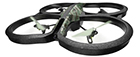
\includegraphics{zalaczniki/obrazy/drony_miniaturki/parrot.jpg} & 50 & 11 \\ \hline
    	    MJX Bugs 3 & 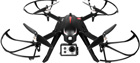
\includegraphics{zalaczniki/obrazy/drony_miniaturki/mjx.jpg} & 300 & 15 \\ \hline
    	    Upair One & 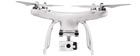
\includegraphics{zalaczniki/obrazy/drony_miniaturki/upair.jpg} & 500 & 20 \\ \hline
    	    Traxxas Aton & 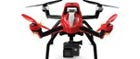
\includegraphics{zalaczniki/obrazy/drony_miniaturki/TRAXXAS.jpg} & 200 & 20 \\ \hline
    	    DJI Phantom 3 Stand & 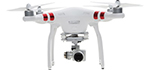
\includegraphics{zalaczniki/obrazy/drony_miniaturki/dji-phantom-3-standard.jpg} & 1500 & 25 \\ \hline
    	    Yuneec Q500+ & 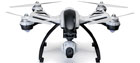
\includegraphics{zalaczniki/obrazy/drony_miniaturki/yuneec.jpg} & 2000 & 22 \\ \hline
    	    3DR Solo & 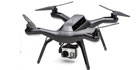
\includegraphics{zalaczniki/obrazy/drony_miniaturki/3dr-solo.jpg} & 500 & 22 \\ \hline
    	    Autel X-Star & 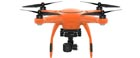
\includegraphics{zalaczniki/obrazy/drony_miniaturki/autel.jpg} & 2000 & 23 \\ \hline
    	    DJI Phantom 3 Pro & 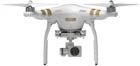
\includegraphics{zalaczniki/obrazy/drony_miniaturki/dji-phantom-3-professional.jpg} & 3000 & 23 \\ \hline
    	    DJI Phantom 4 Pro & 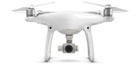
\includegraphics{zalaczniki/obrazy/drony_miniaturki/DJI-Phantom-4.jpg} & 7000 & 26 \\ \hline
    	    DJI Inspire 2 & 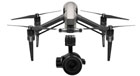
\includegraphics{zalaczniki/obrazy/drony_miniaturki/dji_inspire.jpg} & 7000 & 27 \\ \hline
    	    DJI Mavic Pro & 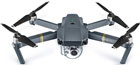
\includegraphics{zalaczniki/obrazy/drony_miniaturki/dji_mavic.jpg} & 7000 & 27 \\ \hline
    \caption{Szacunkowy czas lotu dronów seryjnych \cite{szacunkowyczaslotu}}
    \label{tab:czasLotuDronow}
\end{longtable}

W tabeli zostały wymienione seryjne drony czterowirnikowe, do kwoty $3000\$$ a więc takie które są dostępne od ręki, dla każdego, w sklepie. Można oczywiście latać droższym sprzętem, z baterią o większej gęstości energii, z lepiej zoptymalizowanym sprzętem. Jeżeli zależy nam na zasięgu można też użyć płatowca, płatowcem z takim samym osprzętem i masą startową, polecimy dalej i będziemy latać dłużej. Dla nas czas lotu nie był dużą przeszkodą, misja miała trwać maksymalnie 30 minut, zakładając że czterowirnikowcami nie startujemy od razu, spokojnie wystarczyło nam baterii. Zasięg też nie był problemem, maksymalnie oddalony od miejsca startowego punkt, w którym było jeszcze możliwe znalezienie beaconów, był w odległości około $900 m$ mieliśmy więc pokrycie całego terenu.

\subsection{Zawodność linku telemetrycznego}

Jednym z poważniejszych problemów na jaki się natknąłem, było notoryczne zrywanie linku telemetrycznego pomiędzy dronem a stacją naziemną. Spowodowane to było przede wszystkim tym, że urządzenia które stosowaliśmy były wątpliwej jakości, sytuację pogarszał fakt że musieliśmy mieć jednocześnie kilka linków, do kilku dronów. Link telemtryczny nie jest konieczny do lotu, jest jednak konieczny do wykonania misji, ponieważ po linku telemetrycznym wysyłałem pozycje znalezionych beaconów. Problem rozwiązałem tak, że umożliwiłem wysyłanie pozycji beaconów do stacji naziemnej, przy pomocy sieci telefonii komórkowej GSM, czas takich żądań był dłuższy, ale zwiększyła się niezawodność rozwiązania.

\subsection{Wrażliwość systemu na sytuacje wyjątkowe}

Tak jak wspomniałem wcześniej, nasz system był wrażliwy na różne wyjątkowe sytuacje, takie jak nagła zmiana pogody, opady deszczu, silny wiatr, nie posiadaliśmy również czujników zbliżeniowych na dronach, każdy więc błąd operatora mógł doprowadzić do kolizji z przeszkodą. 

\subsection{Problemy sprzętowe}

Nie ominęły nas również problemy sprzętowe, wspominałem już o modułach telemetrycznych wątpliwej jakości. Podczas konkursu mieliśmy też problem z modułem GPS w jednym z dronów. Zawodziły też inne mniejsze podzespoły, mieliśmy jednak dużo sprzętu na wymianę.

\subsection{Sygnał beacona}

Pierwsza sprawa jest taka, że sygnał nadawany przez beacony miał doświadczalnie przez nas zmierzony zasięg maksymalny około $80 m$, przy dobrych warunkach pogodowych i bezpośredniej widoczności, bez żadnych przeszkód pomiędzy odbiornikiem i nadajnikiem. Dodatkowo opieraliśmy się tutaj na parametrze sygnału, RSSI \cite{rssi}, który wskazuje na siłę sygnału jaką widzi urządzenie odbiorcze, wskaźnik ten bardzo zależy od warunków pogodowych, przeszkód pomiędzy urządzeniami, wreszcie od samego wykonania urządzeń, szczególnie odbiorczego, na jego podstawie jedynie w przybliżeniu mogliśmy określić czy znajdujemy się w pobliżu beacona, czy jesteśmy daleko. Żeby więc znaleźć takiego beacona na ziemi z powietrza musimy po pierwsze lecieć nisko, a czasami nie jest to możliwe, są drzewa, budynki, linie energetyczne, które nie pozwolą nam lecieć nisko, załóżmy więc że na wysokości powyżej 20 metrów mamy wolną przestrzeń. Żeby jednak znaleźć wszystkie beacony, musimy lecieć tak, żeby każdy punkt oblatywanego obszaru był od nas najdalej o te założone kilkadziesiąt metrów, skoro maksymalnie widzieliśmy beacona z $80 m$ założyliśmy że musimy lecieć co najdalej $60 m$ od każdego punktu na przeszukiwanym obszarze. Im wyżej lecimy tym musimy lecieć ciaśniej, czyli nasze ścieżki muszą być bliżej siebie. Problem ilustruje rysunek \ref{fig:schematprzelotu}.

\begin{figure}[!th]
    \centering
    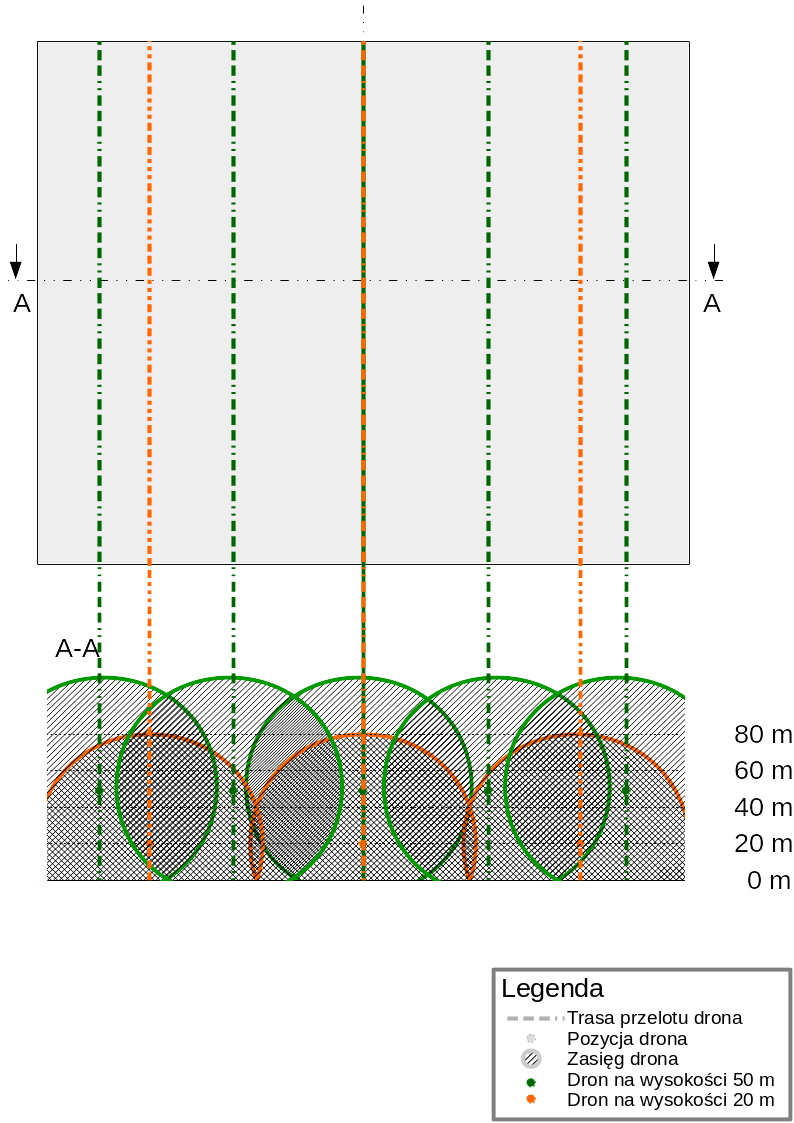
\includegraphics[width=15cm]{zalaczniki/obrazy/schemat_przelotu.png}
    \caption{Schematy przelotu dla różnych wysokości nad gruntem}
    \label{fig:schematprzelotu}
\end{figure}

Na rysunku widzimy przykładowy obszar który musimy zbadać i dwie proponowane wysokości przelotu, wysokość $50 m$ oznaczona jest na zielono, wysokość $20 m$ na pomarańczowo, widać że aby przelecieć zadany obszar na wysokości $50 m$ musimy przelecieć go w sumie 5 razy, w przypadku lotu na wysokości $20 m$ wystarczy 3 razy, lot na wysokości $60 m$ lb wyżej, przy naszych założeniach nie miałby już sensu.

\section{Testy i misja konkursowa}

Testy pojedynczych modułów przeprowadzane były na bieżąco, testów integracyjnych było jednak stosunkowo mało, ze względów logistycznych, ciężko znaleźć odpowiednie miejsce do latania, trzeba zabierać ze sobą dużo sprzętu. Tak na prawdę pierwszym prawdziwym sprawdzianem z wykonania misji była misja konkursowa. Poszła nam ona całkiem dobrze, nie wystrzegliśmy się jednak błędów, wylecieliśmy poza dozwolony obszar, nie udało nam się znaleźć jednego beacona, a dokładność naszych pomiarów pozostawiała wiele do życzenia. Dodatkowo aplikacja przez jakiś czas odpowiadała ze sporym opóźnieniem i musieliśmy sobie z tym radzić, przyczyny opóźnienia nie udało mi się ustalić. 

Aplikacja do aproksymacji musiała znać przybliżoną charakterystykę sygnału beaconów, testy takie zostały przez nas wykonane, a wyniki zaimplementowane w funkcji aproksymującej. Aproksymacja działała całkiem dobrze, nie dało się jednak zaufać jej w pełni, operator systemu musiał na bieżąco weryfikować dane, pojawiające się na pulpicie systemu.

Na pierwszym obrazku w tym rozdziale \ref{fig:beaconykonkursowe} widzimy miejsca w których organizatorzy umieścili beacony, oczywiście nie znaliśmy ich położenia przed konkursem, dopiero po zakończeniu konkursu otrzymaliśmy te pozycje. Gwiazdkami w kolorach systemu triage, oznaczone są kolejne beacony, etykieta pod gwiazdką wskazuje na bajty Major i Minor nadawane przez beacony.

\begin{figure}[!th]
    \centering
    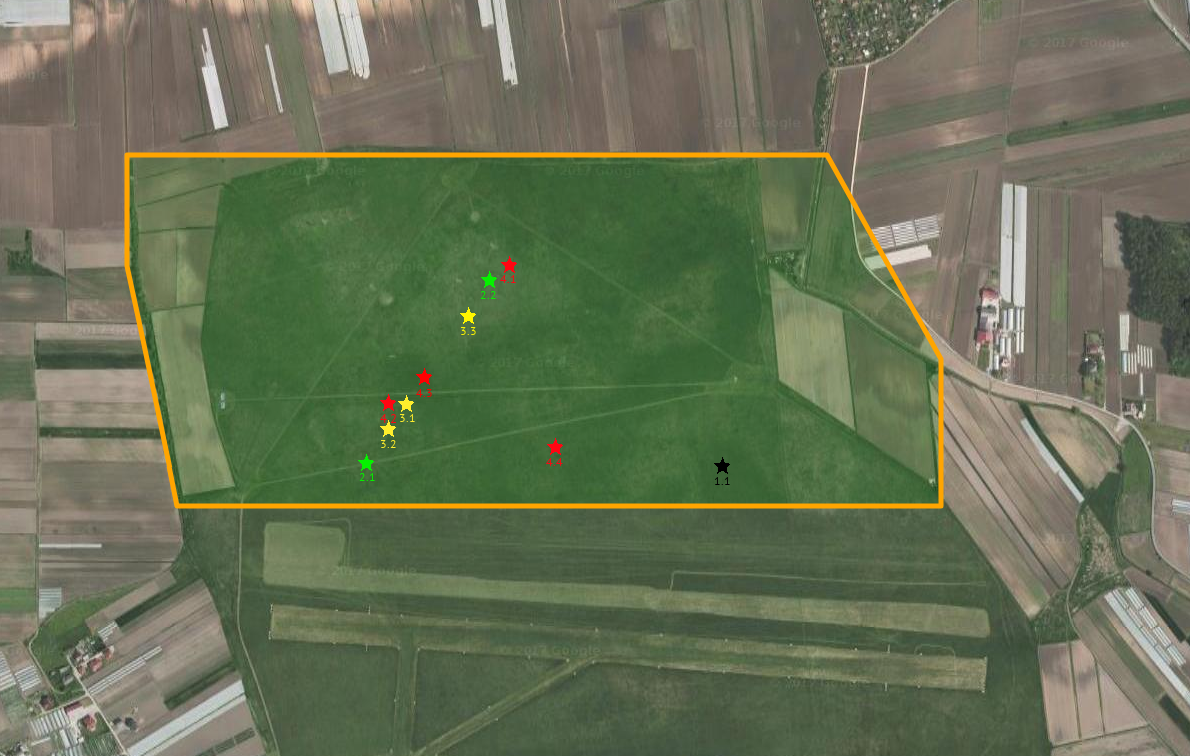
\includegraphics[width=15cm]{zalaczniki/obrazy/beacony_konkursowe.png}
    \caption{Pozycje beaconów rozmieszczonych przez organizatorów podczas konkursu}
    \label{fig:beaconykonkursowe}
\end{figure}

Kolejne zdjęcie \ref{fig:wskazanieczerwone} przedstawia, jak wyglądało wskazanie systemu na miejsce położenia beaconów nadających bajt Major równy 4. Udało nam się znaleźć wszystkie czerwone beacony, z dość dobrą dokładnością, chociaż nie ukrywam że niektóre pomiary były mylące, a nasz system nie miał niestety zbyt dużych możliwości filtracji danych, widać to na przykładzie beacona 4.1, otrzymaliśmy sprzeczne dane, jakoby beacon nadający te dane znajdował się w dwóch miejscach, oddalonych od siebie o około $300 m$, co nie było możliwe, bo tak jak wspominałem, zasięg sygnału beaconów to maksymalnie około $80 m$.

\begin{figure}[!th]
    \centering
    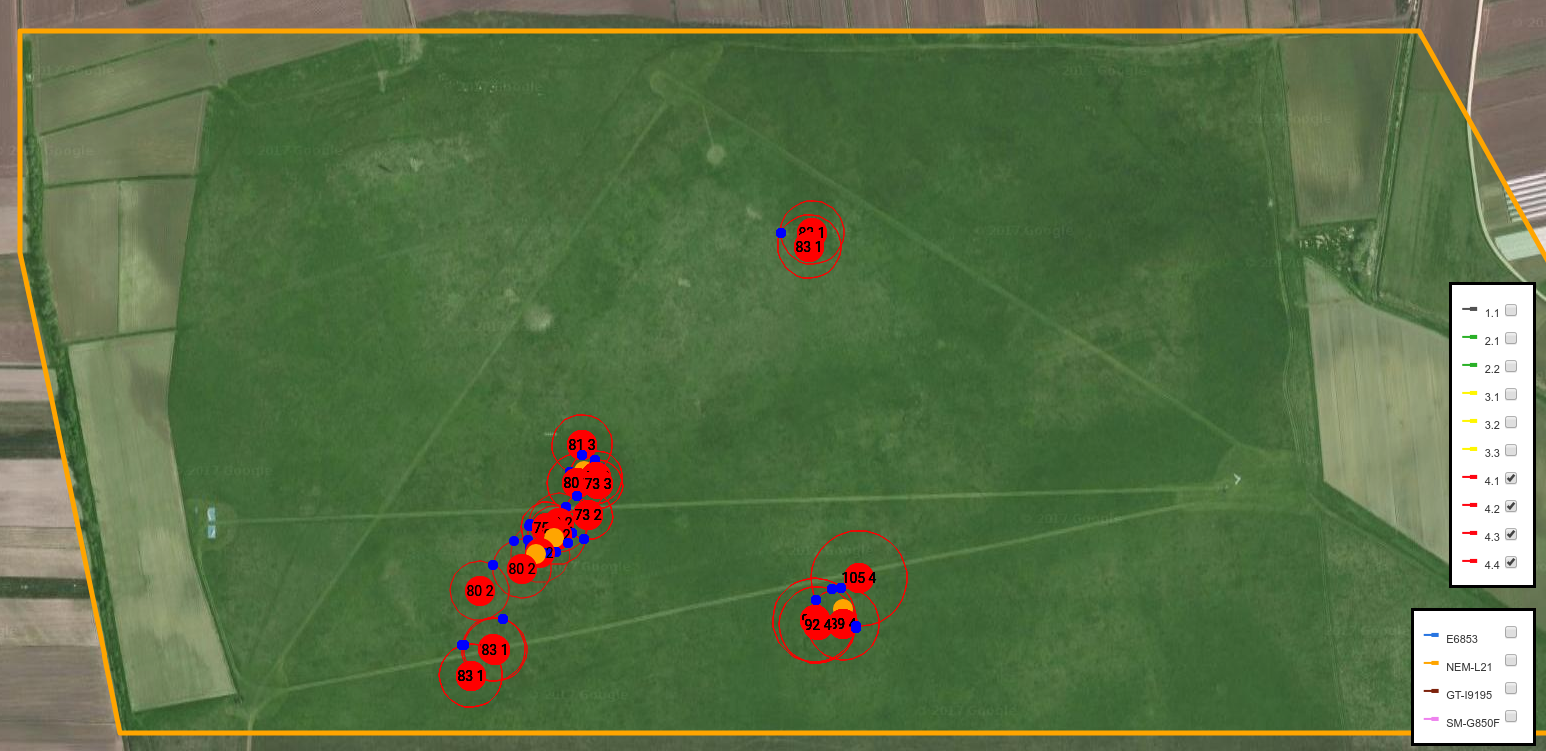
\includegraphics[width=15cm]{zalaczniki/obrazy/wskazanie_czerwone.png}
    \caption{Wskazanie naszego systemu na miejsca położenia beaconów czerownych}
    \label{fig:wskazanieczerwone}
\end{figure}

Następny rysunek \ref{fig:wskazaniezolte} pokazuje wskazanie na żółte beacony, jak przy czerwonych mieliśmy w miarę dobrą dokładność, w najgorszym przypadku $22,37 m$ tak w przypadku żółtego z numerem 3 pomyliliśmy się aż o $126,74 m$, to był nasz najgorszy wynik, żółty z numerem 2 miał błąd $81,58 m$, widać że potrzebna byłaby dodatkowa praca nad polepszeniem dokładności pomiarów.

\begin{figure}[!th]
    \centering
    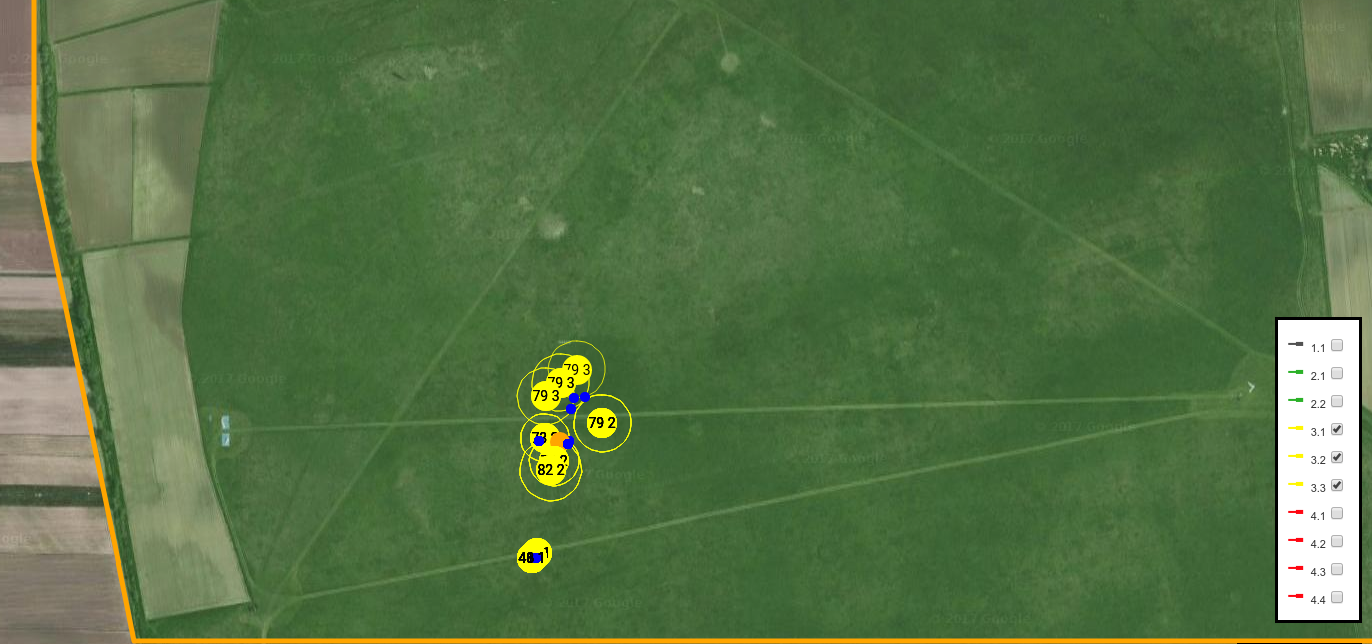
\includegraphics[width=15cm]{zalaczniki/obrazy/wskazanie_zolte.png}
    \caption{Wskazanie naszego systemu na miejsca położenia beaconów żółtych}
    \label{fig:wskazaniezolte}
\end{figure}

Ostatnie są beacony zielone, czarnego niestety nie znaleźliśmy, na rysunku \ref{fig:wskazaniezielone} widzimy nasze wskazanie na nie. Dokładności w tym przypadku były w miarę dobre, w okolicach $15 m$.

\begin{figure}[!th]
    \centering
    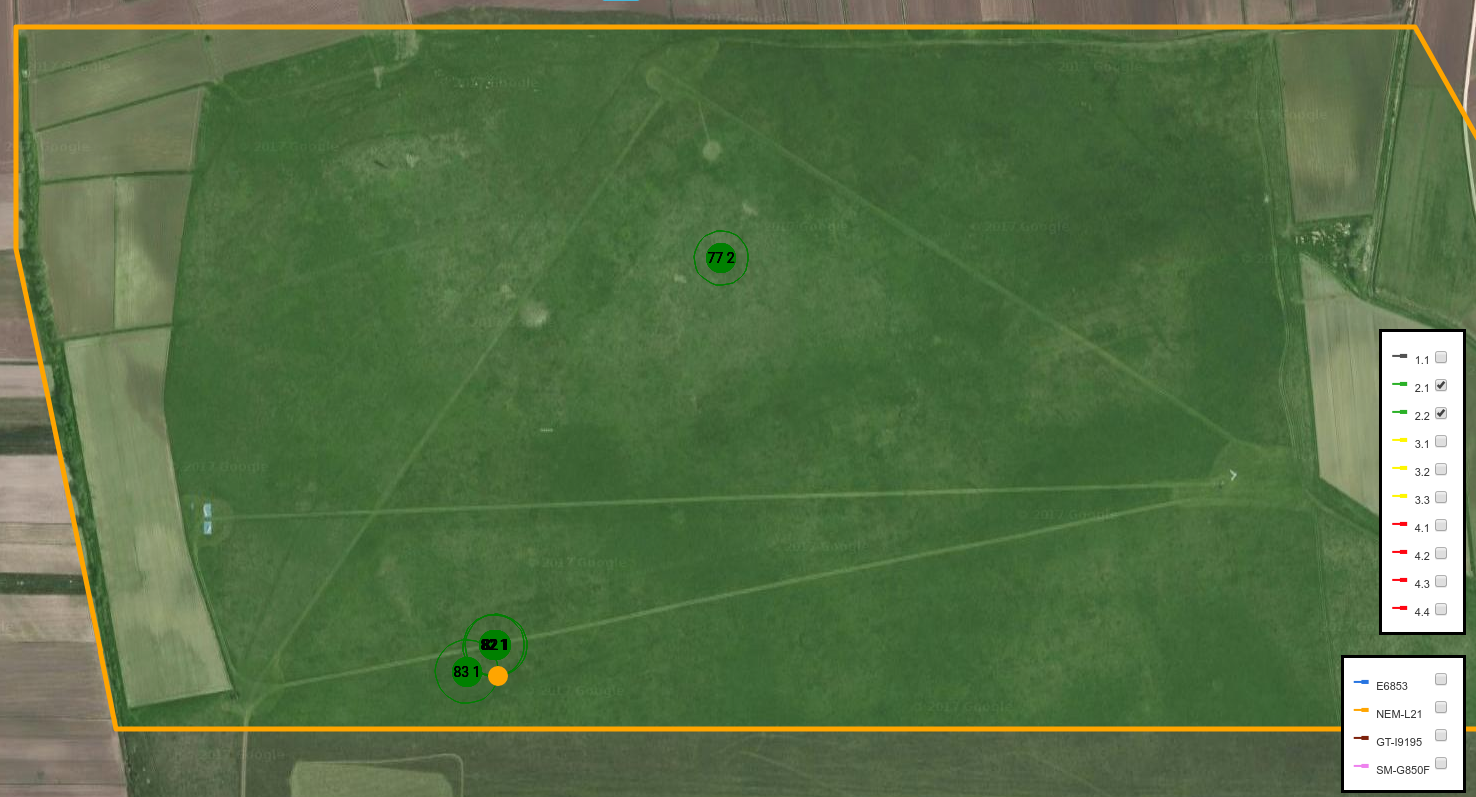
\includegraphics[width=15cm]{zalaczniki/obrazy/wskazanie_zielone.png}
    \caption{Wskazanie naszego systemu na miejsca położenia beaconów zielonych}
    \label{fig:wskazaniezielone}
\end{figure}

Na ostatnim rysunku \ref{fig:beaconykonkursowenasze} mamy porównanie tego gdzie były beacony do tego co wskazał mój system.

\begin{figure}[!th]
    \centering
    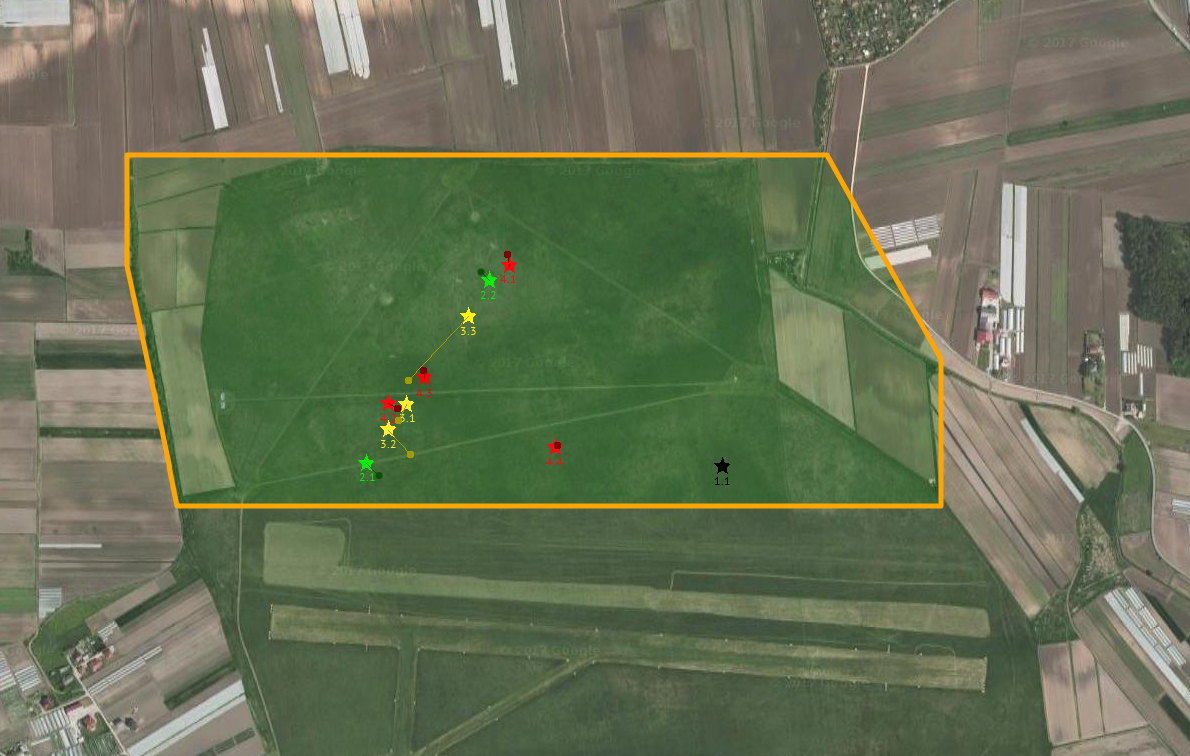
\includegraphics[width=15cm]{zalaczniki/obrazy/beacony_konkursowe_nasze.png}
    \caption{Nałożenie naszych szacunkowych pozycji na obraz z pozycjami realnymi}
    \label{fig:beaconykonkursowenasze}
\end{figure}

Na koniec tabela \ref{tab:polozeniebeaconowiblad} z położeniem beaconów, naszym wskazaniem i naszym błędem pomiaru.

\begin{tablica}
    {Położenie beaconów konkursowych oraz naszych i błąd naszego pomiaru}
    {Położenie beaconów konkursowych oraz naszych i błąd naszego pomiaru}
    {
    \begin{tabular}{|c|c|c|c|} \hline
	    \textbf{Beacon} & \textbf{Pozycja realna [lat, lon]} & \textbf{Pozycja zmierzona [lat, lon]} & \textbf{Błąd [m]} \\ \hline
	    1.1 & 50.0888040, 20.2041863 & & \\ \hline
	    2.1 & 50.0889409, 20.1968885 & 50.088867, 20.197039 & 13,46 \\ \hline
	    2.2 & 50.0916493, 20.1993463 & 50.091776, 20.199251 & 16,65 \\ \hline
	    3.1 & 50.0898048, 20.1971456 & 50.089800, 20.197217 & 4,73 \\ \hline
	    3.2 & 50.0896552, 20.1971186 & 50.089036, 20.197759 & 81,58 \\ \hline
	    3.3 & 50.0908825, 20.1989062 & 50.089979, 20.197821 & 126,74 \\ \hline
	    4.1 & 50.0916549, 20.1998945 & 50.091767, 20.199826 & 13,61 \\ \hline
	    4.2 & 50.0897875, 20.1975500 & 50.089981, 20.197523 & 22,37 \\ \hline
	    4.3 & 50.0900354, 20.1976396 & 50.090101, 20.197607 & 8,21 \\ \hline
	    4.4 & 50.0890267, 20.2006400 & 50.089051, 20.200665 & 3,23 \\ \hline
   \end{tabular}
    }
    \label{tab:polozeniebeaconowiblad}
\end{tablica}

\section{Podsumowanie}

\subsection{Wnioski}

Podstawowym wnioskiem z przeprowadzonych testów i zawodów jest to że system w takim stanie w jakim był, nie może mieć żadnego poważnego zastosowania, w szczególności nie może służyć ratownikom przy prowadzeniu akcji ratowniczej. Drony które mieliśmy do dyspozycji miały krótkie czasy lotu, mały zasięg, a prawdziwa misja ratunkowa nie odbywa się na powierzchni kilku kilometrów kwadratowych, gdzie można całą akcję przeprowadzić ręcznie, bez użycia niepotrzebnego dodatkowego sprzętu. Można oczywiście użyć droższego sprzętu, o większym zasięgu, ale znów czy beacony to dobry wybór? Moim zdaniem nie, ratownik który oznacza poszkodowanego beaconem, równie dobrze może sam zaznaczyć na mapie gdzie go zostawił, nie są tu potrzebne drony do skanowania obszaru. Kolejną sprawą jest to, że nasz system zakłada że beacony leżą statycznie w jednym miejscu, w prawdziwym życiu człowiek może się ruszać i przechodzić w inne miejsce, a to eliminuje ten system z użytku.

\subsection{Plany na przyszłość}

Planów na przyszłość z tym konkretnym projektem nie mam, wydaje mi się że to co tutaj robiliśmy, w tej formie, nie ma przyszłości w ratownictwie, co najwyżej komponenty tego systemu mogłyby mieć zastosowanie w innym projekcie. Samo wyszukiwanie beaconów mogłoby mieć zastosowanie na przykład w biurach do sprawdzania kiedy pracownik przyszedł, wyszedł, gdzie mniej więcej się znajduje, a można by to było realizować przy pomocy beacona takiego jak na rysunku \ref{fig:beaconcard}.

\begin{figure}[!th]
    \centering
    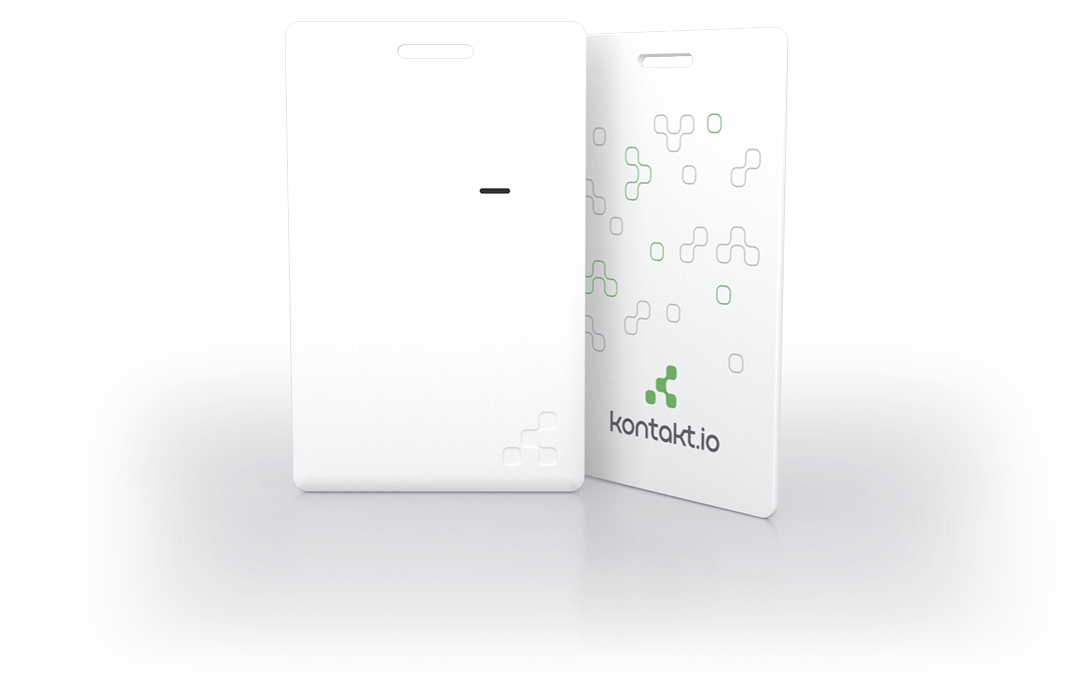
\includegraphics[width=15cm]{zalaczniki/obrazy/beacon_card.png}
    \caption{Beacon w postaci karty, rozmiarowo zlbiżony do karty kredytowej}
    \label{fig:beaconcard}
\end{figure}

Podobnie na imprezach masowych można przy pomocy takiego beacon śledzić osoby. Gdyby zasięg sygnału takiego beacona był większy, na przykład kilka kilometrów, takie beacony można by było rozdawać ludziom którzy idą w góry, dzięki temu łatwiej byłoby ich później znaleźć przy pomocy drona, w przypadku gdyby zabłądzili.
